\documentclass{beamer}

% german content
\usepackage[ngerman]{babel}

%for Lisas PC
\usepackage[T1]{fontenc}
\usepackage[latin1]{inputenc}

% bibliography
\usepackage[
backend=biber,
style=authoryear,
citestyle=authoryear,
autocite=footnote
]{biblatex}
\addbibresource{bibliography.bib}

% images
\usepackage{graphicx}
\graphicspath{ {./images/} }

\title{Import/Export von saisonalen Produkten}
% \subtitle{}
\author[Dao, Gabele, Neidel, Neuthor, Spannbauer, Wiegandt]{
  Dao, Duc Trung \and\\
  Gabele, Jörg \and\\
  Neidel, Jonathan \and\\
  Neuthor, Marco \and\\
  Spannbauer, Daniel \and\\
  Wiegandt, Lisa-Marlen
}
\date{Januar 2021}
\institute{HTW Berlin, Angewandte Informatik}
\logo{
\includegraphics[width=1cm]{logo}}

% theme + color theme
\usetheme{Szeged}
\usecolortheme{whale}
% see: https://deic-web.uab.cat/~iblanes/beamer_gallery/index.html

\begin{document}
\frame{\titlepage}

\begin{frame}
	\frametitle{Abstract}
	Betrachtung der Auswirkungen von Produktsaisons auf dessen Import und Export
	\begin{itemize}
		\item Steigt der Preis?
		\item Muss sogar verstärkt importiert werden?
	\end{itemize}
\end{frame}

% show all section names
\begin{frame}
\frametitle{Inhalt}
\tableofcontents
\end{frame}
% how to exclude a section from toc: https://tex.stackexchange.com/a/66633


\section{Organisation}

\begin{frame}
	\begin{center}
	{\Huge Organisation}
	\end{center}
\end{frame}

\begin{frame}
	\frametitle{Rollenverteilung}
	\begin{description}
		\item[Duc Trung Dao, 575477]Main Data Seeker and Preprocessor
		\item[Jörg Gabele, 571127]Master of Theorie
		\item[Jonathan Neidel, 573619]Projekt Manager
		\item[Marco Neuthor, 573738]Principal Visualizer
		\item[Daniel Spannbauer, 572836]Head of Data Processing
		\item[Lisa-Marlen Wiegandt, 572770]Editor of Chief
	\end{description}
    \end{frame}

\section{Definitionen}
\begin{frame}
	\begin{center}
		{\Huge Definitionen}
	\end{center}
\end{frame}

\section{Datenbeschaffung und -bereinigung}
\begin{frame}
	\begin{center}
		{\Huge Datenbeschaffung}
	\end{center}
\end{frame}

\begin{frame}
	\frametitle{Beginn der Datensuche}
		\begin{itemize}
			\item statistische Jahrbuch des Bundesministeriums für Ernährung und Landwirtschaft (BMEL)
		\end{itemize}

		\begin{figure}[!tbp]
  			\centering
			\begin{minipage}[b]{0.3\textwidth}
    			
\includegraphics[scale=0.15, width=\textwidth]{1_BMEL-Statistisches_Jahrbuch}
  			\end{minipage}
  		\hfill
			\begin{minipage}[b]{0.4\textwidth}
    			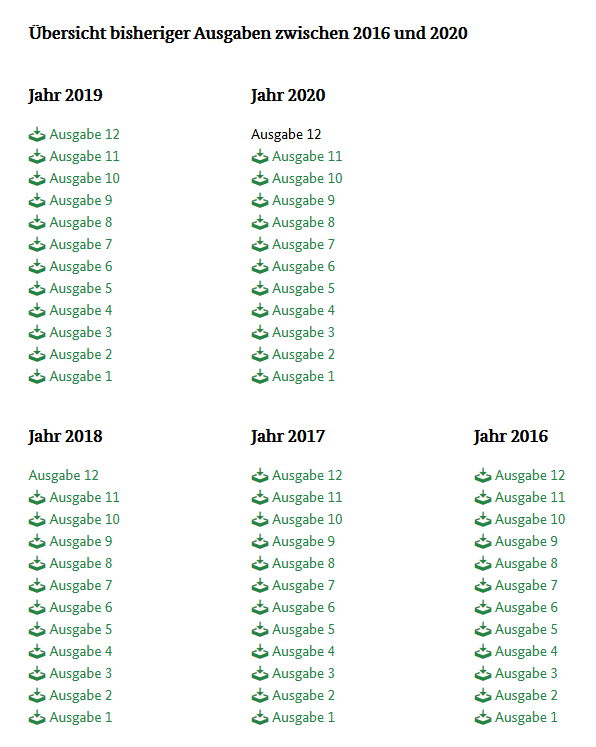
\includegraphics[scale=0.4,width=\textwidth]{2_Monatsberichte}
  			\end{minipage}
		\end{figure}
\end{frame}

\begin{frame}
	\frametitle{Beginn der Datensuche}
	\begin{figure}[h]
	\caption{Beispieltabelle aus dem statistischen Jahrbuch}
	\centering
	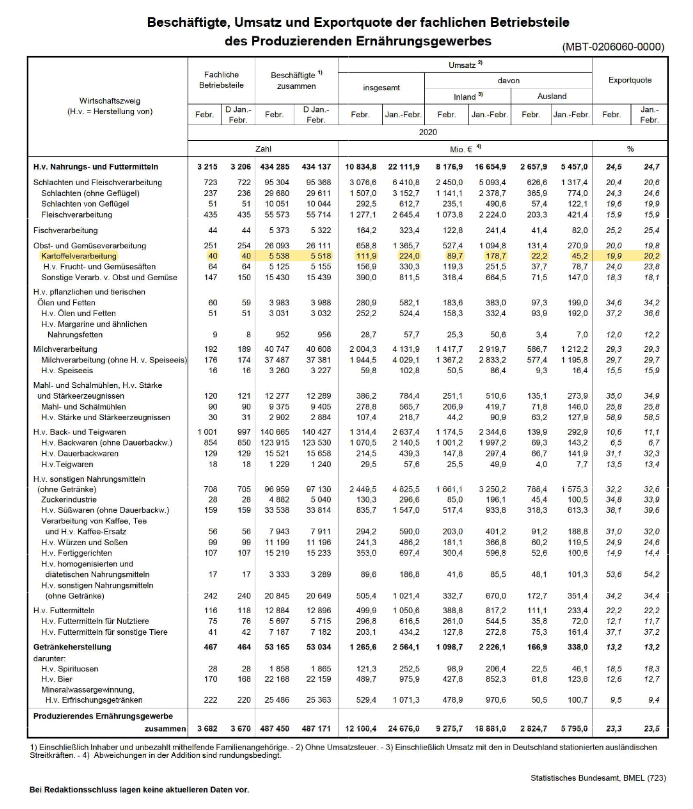
\includegraphics[scale=0.5]{3_Beispieltabelle}
		%Größe mit Daniel noch besprechen und Quellen einfügen
	\end{figure}
\end{frame}

\begin{frame}
	\frametitle{Probleme}
	\begin{itemize}
		\item Informationen per Hand exportiert
		\item unvollständiger Datensatz
	\end{itemize}
\end{frame}

\begin{frame}
	\frametitle{Probleme}
	\begin{figure}[h]
		\caption{unvollständige Auflistung}
		\centering
		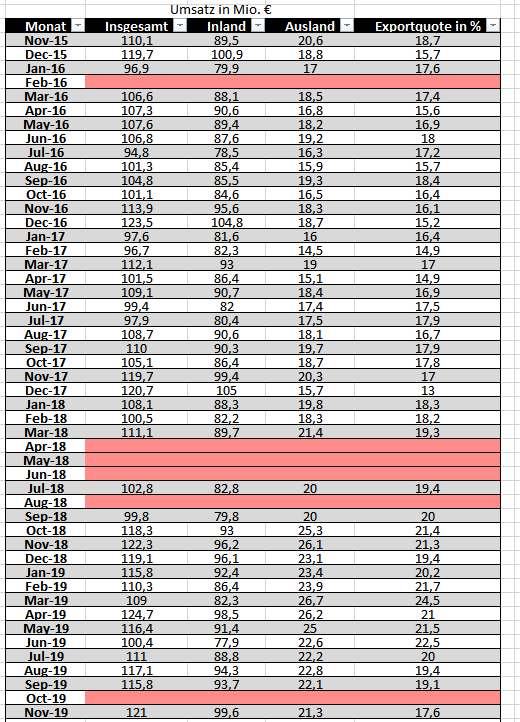
\includegraphics[scale=0.3]{4_Monatsberichte_unvoll}
	\end{figure}
\end{frame}

\begin{frame}
	\frametitle{Weitere Suche}
	\begin{itemize}
		\item statista.com
			\begin{itemize}
				\item simple Statistiken
				\item einzelne Diagramme
			\end{itemize}
	\end{itemize}
\end{frame}

\begin{frame}
	\frametitle{statista.com}
	\begin{figure}[h]
		\caption{Beispieltabelle von statista.com}
		\centering
		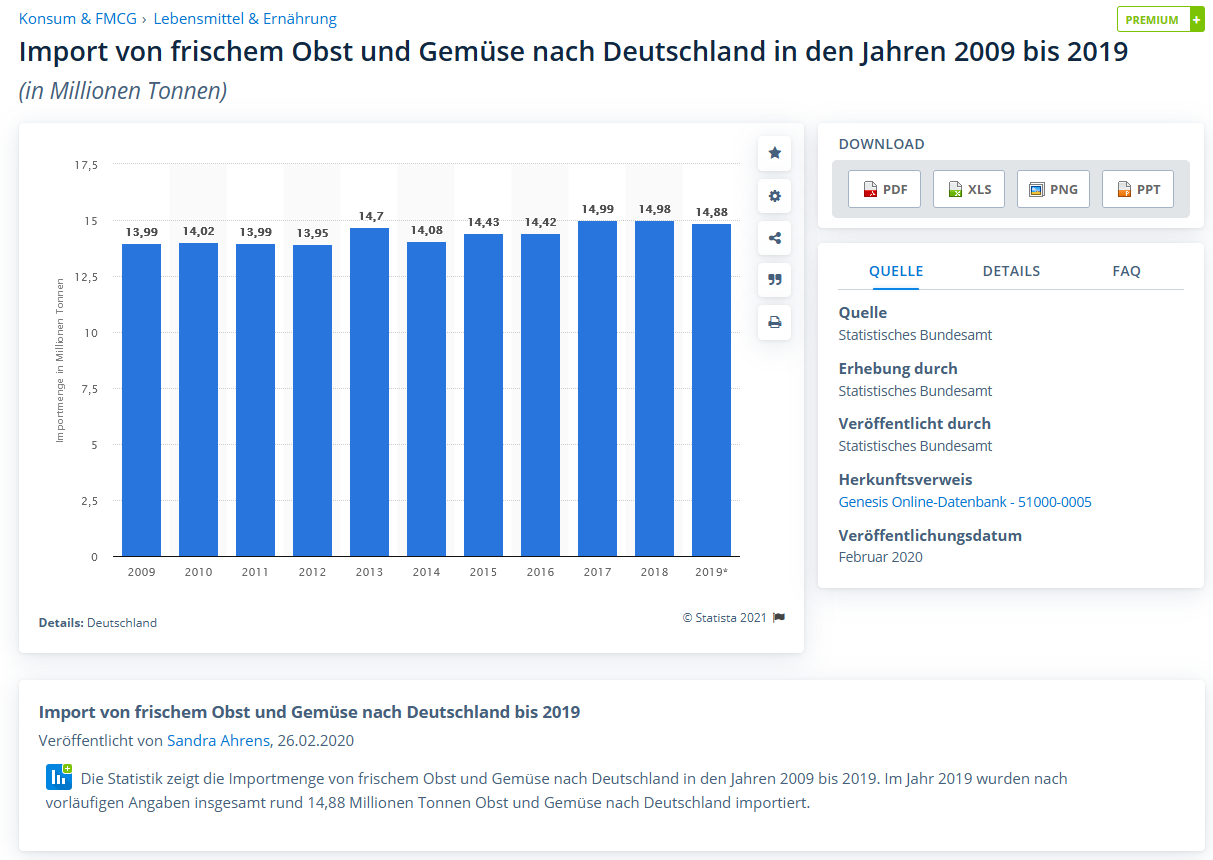
\includegraphics[scale=0.3]{5_Destatis_Report}
	\end{figure}
\end{frame}

\begin{frame}
	\frametitle{statista.com}
	\begin{figure}[h]
		\caption{Beispieltabelle von statista.com}
		\centering
		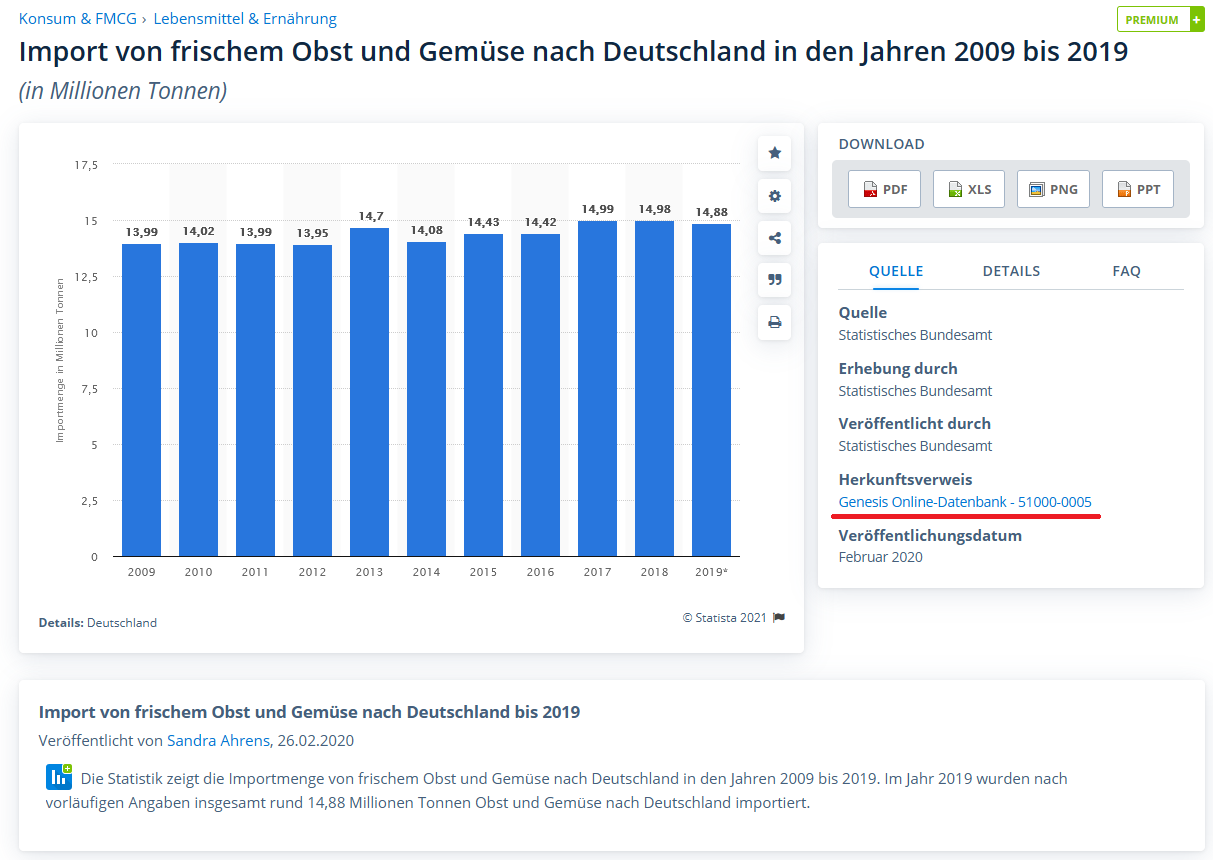
\includegraphics[scale=0.3]{5_Destatis_Report_highlightet}
	\end{figure}
\end{frame}  

\begin{frame}
	\frametitle{Lösungen}
	\begin{figure}[h]
		\caption{Startseite der Genesis-Website}
		\centering
		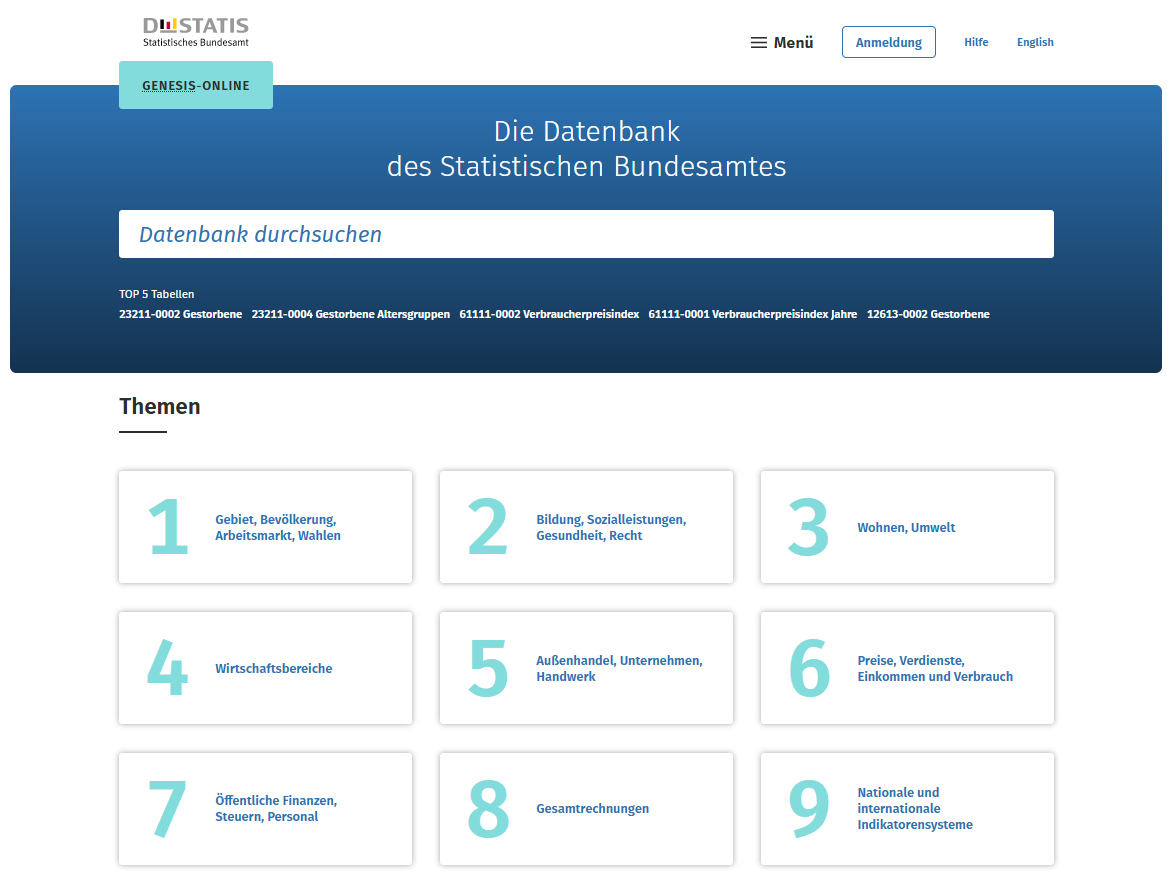
\includegraphics[scale=0.15]{6_Denesis_Destatis}
	\end{figure}
\end{frame}

\begin{frame}
	\frametitle{Lösung}
	\begin{figure}[h]
		\caption{Auszug der Tabellenübersicht von Genesis}
		\centering
		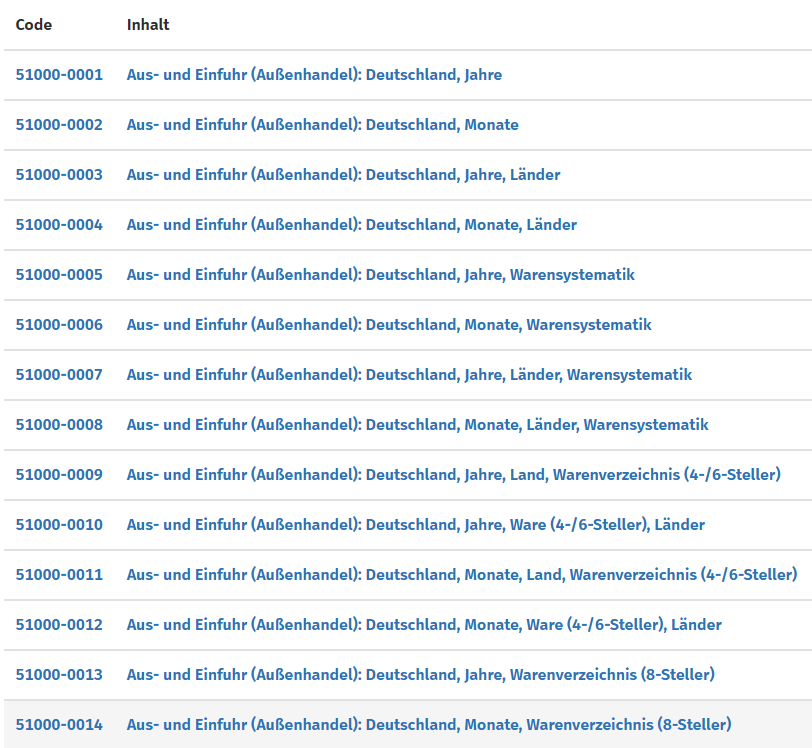
\includegraphics[scale=0.2]{8_Tabellen_codes}
	\end{figure}
\end{frame}

\begin{frame}
	\frametitle{}
	\begin{figure}[h]
		\caption{Datensatz Generierung auf der Genesis Website}
		\centering
		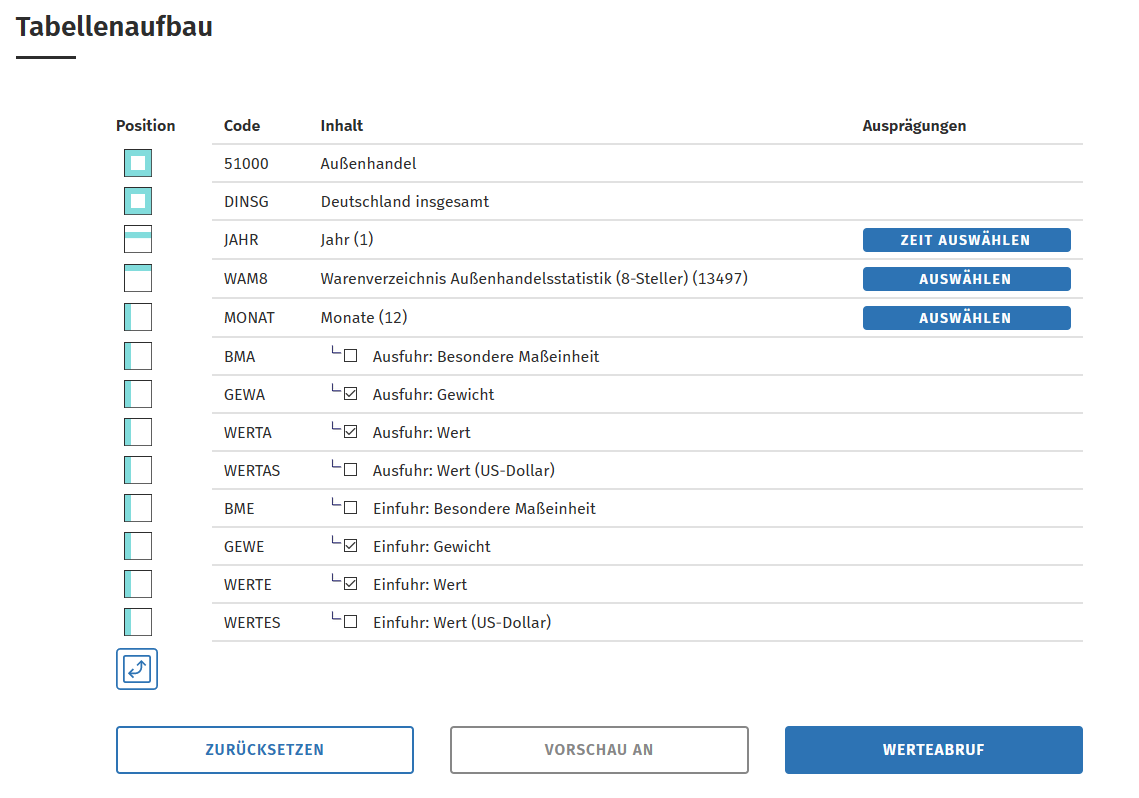
\includegraphics[scale=0.25]{9_Tabellanaufbau}
	\end{figure}
\end{frame}

\begin{frame}
	\frametitle{Lösung}
	\begin{itemize}
		\item Import in Excel
		\item anschließend grobe Aufbereitungsschritte in kleinere CSV-Dateien
	\end{itemize}
\end{frame}

\section{Datenverarbeitung}
\begin{frame}
	\begin{center}
		{\Huge Datenverarbeitung}
	\end{center}
\end{frame}

\begin{frame}
	\frametitle{Datenstruktur}
	\begin{figure}[b]
		\centering
		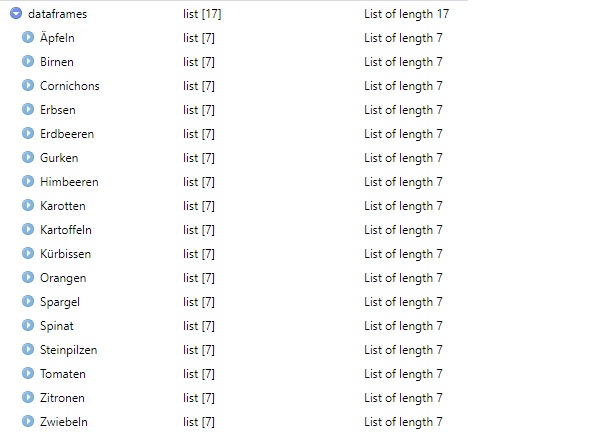
\includegraphics[scale=0.6]{Marco_1_Folie_1}
	\end{figure}
\end{frame}

\begin{frame}
	\frametitle{Datenstruktur}
	\begin{figure}[b]
		\centering
		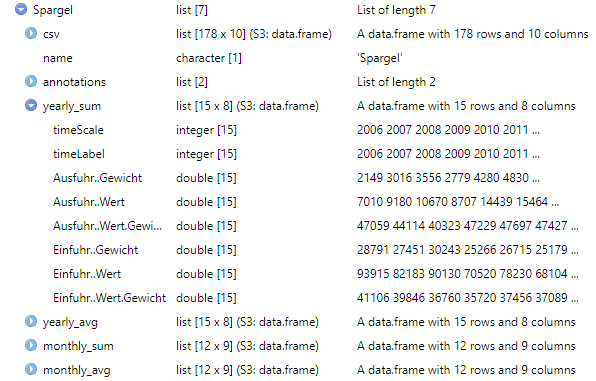
\includegraphics[scale=0.6]{Marco_1_Folie_2}
	\end{figure}
\end{frame}

\begin{frame}
	\frametitle{Probleme der Darstellung}
	\begin{itemize}
		\item diskrete Daten an der Abszisse
		\begin{itemize}
			\item falsche Aussagen aus Liniendigramm 
		\end{itemize}
		\item optische Abgrenzung schwierig
		\item Saisons nicht erkennbar
	\end{itemize}

	\begin{figure}[b]
		\centering
		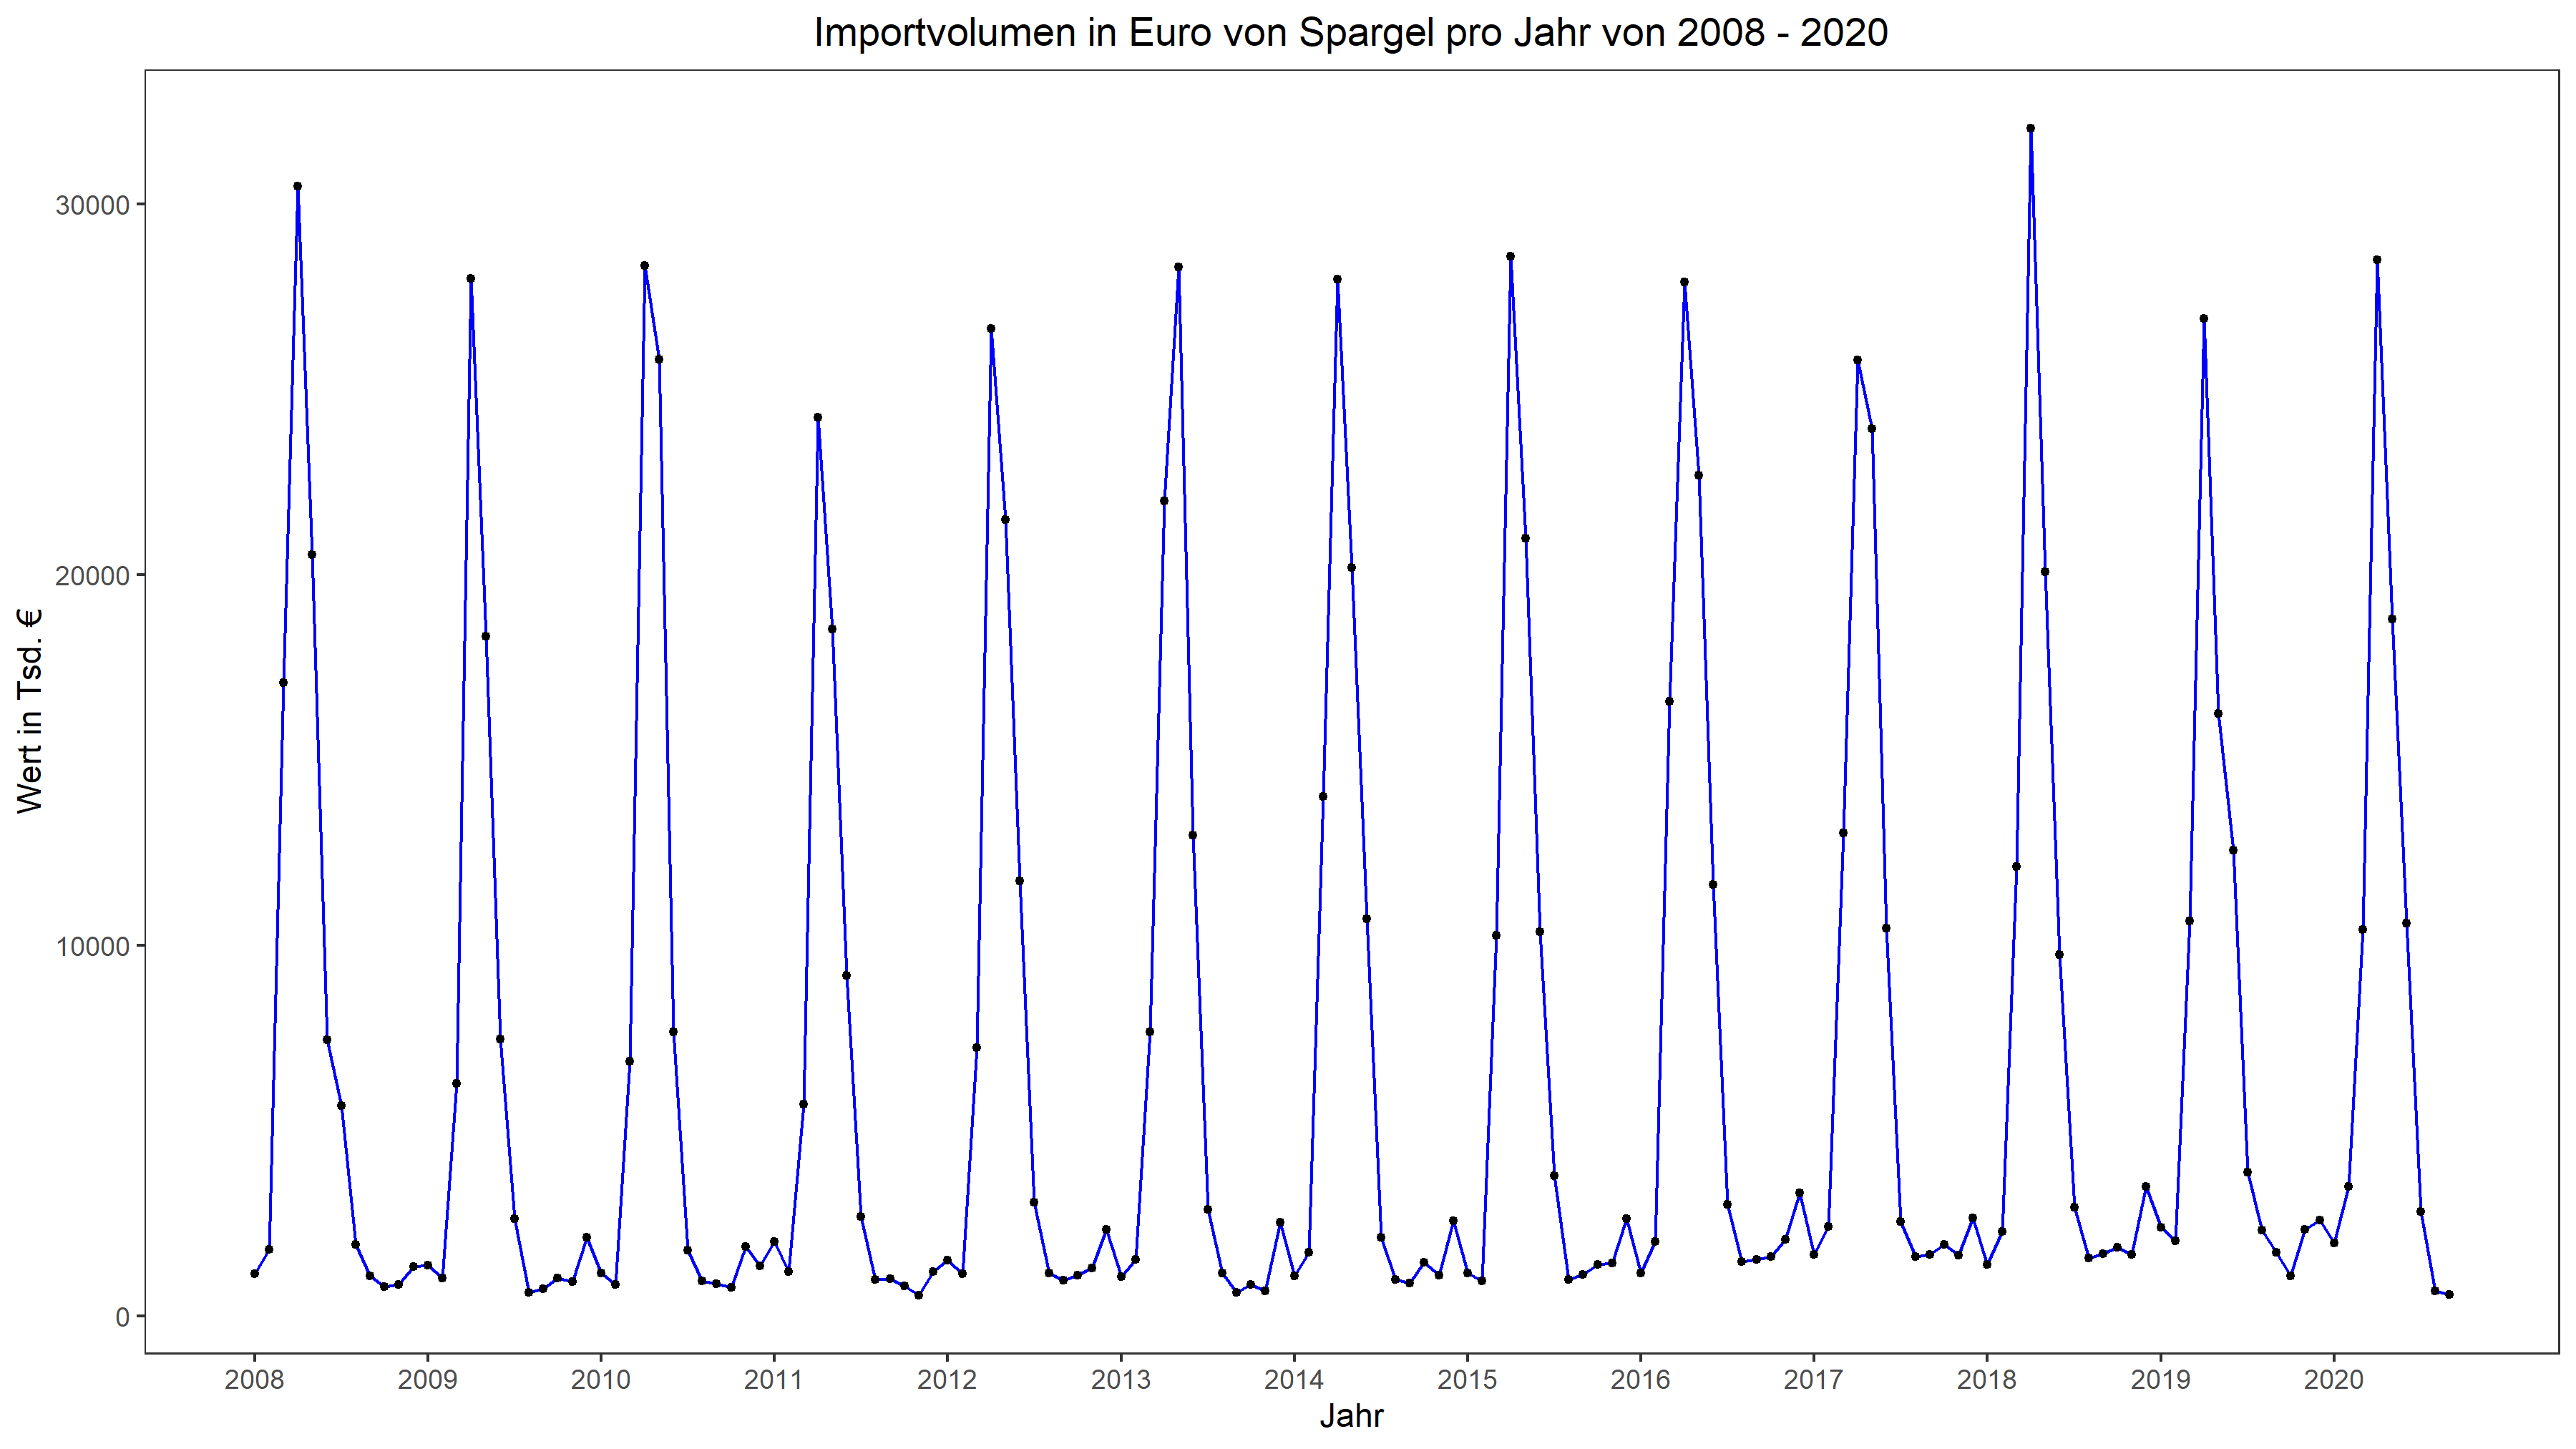
\includegraphics[scale=0.3]{Marco_2_Folie}
	\end{figure}
\end{frame}

\begin{frame}
	\frametitle{Darstellung der Saison}
	\begin{figure}
		\centering
		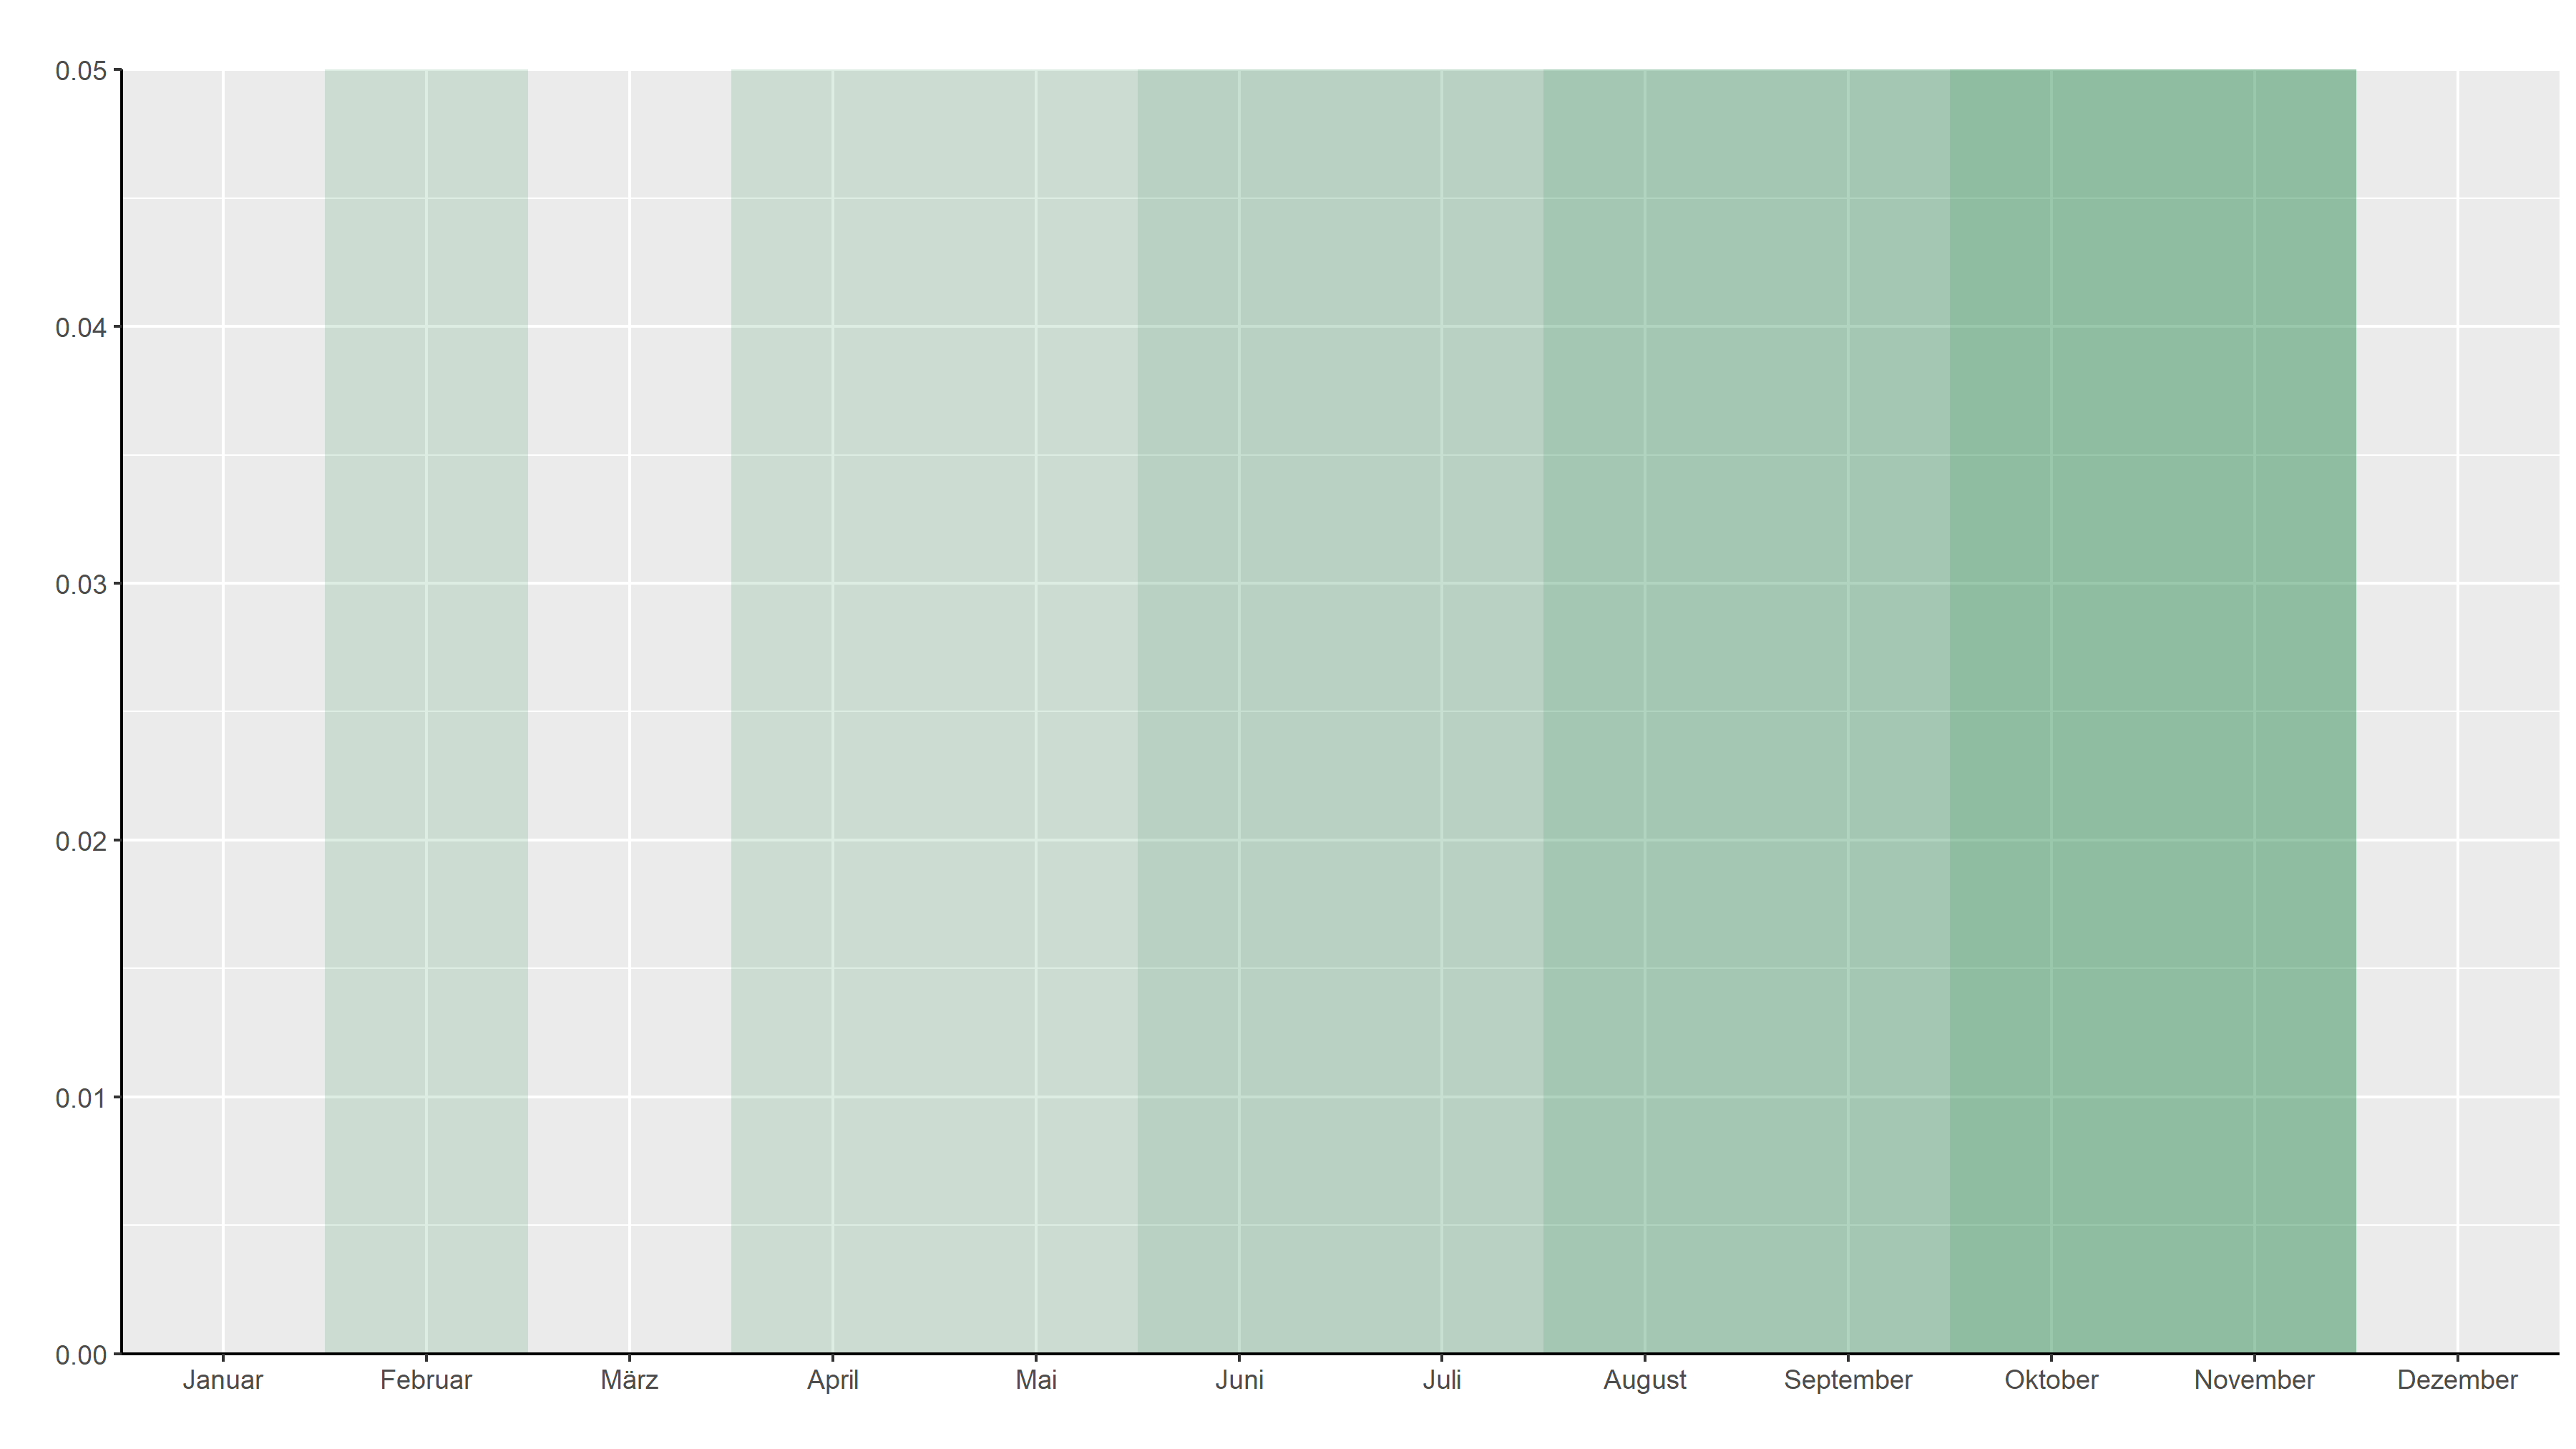
\includegraphics[scale=0.35]{Marco_3_Folie}
	\end{figure}
\end{frame}

\begin{frame}
	\frametitle{optimierte Darstellung}
	\begin{figure}[b]
		\centering
		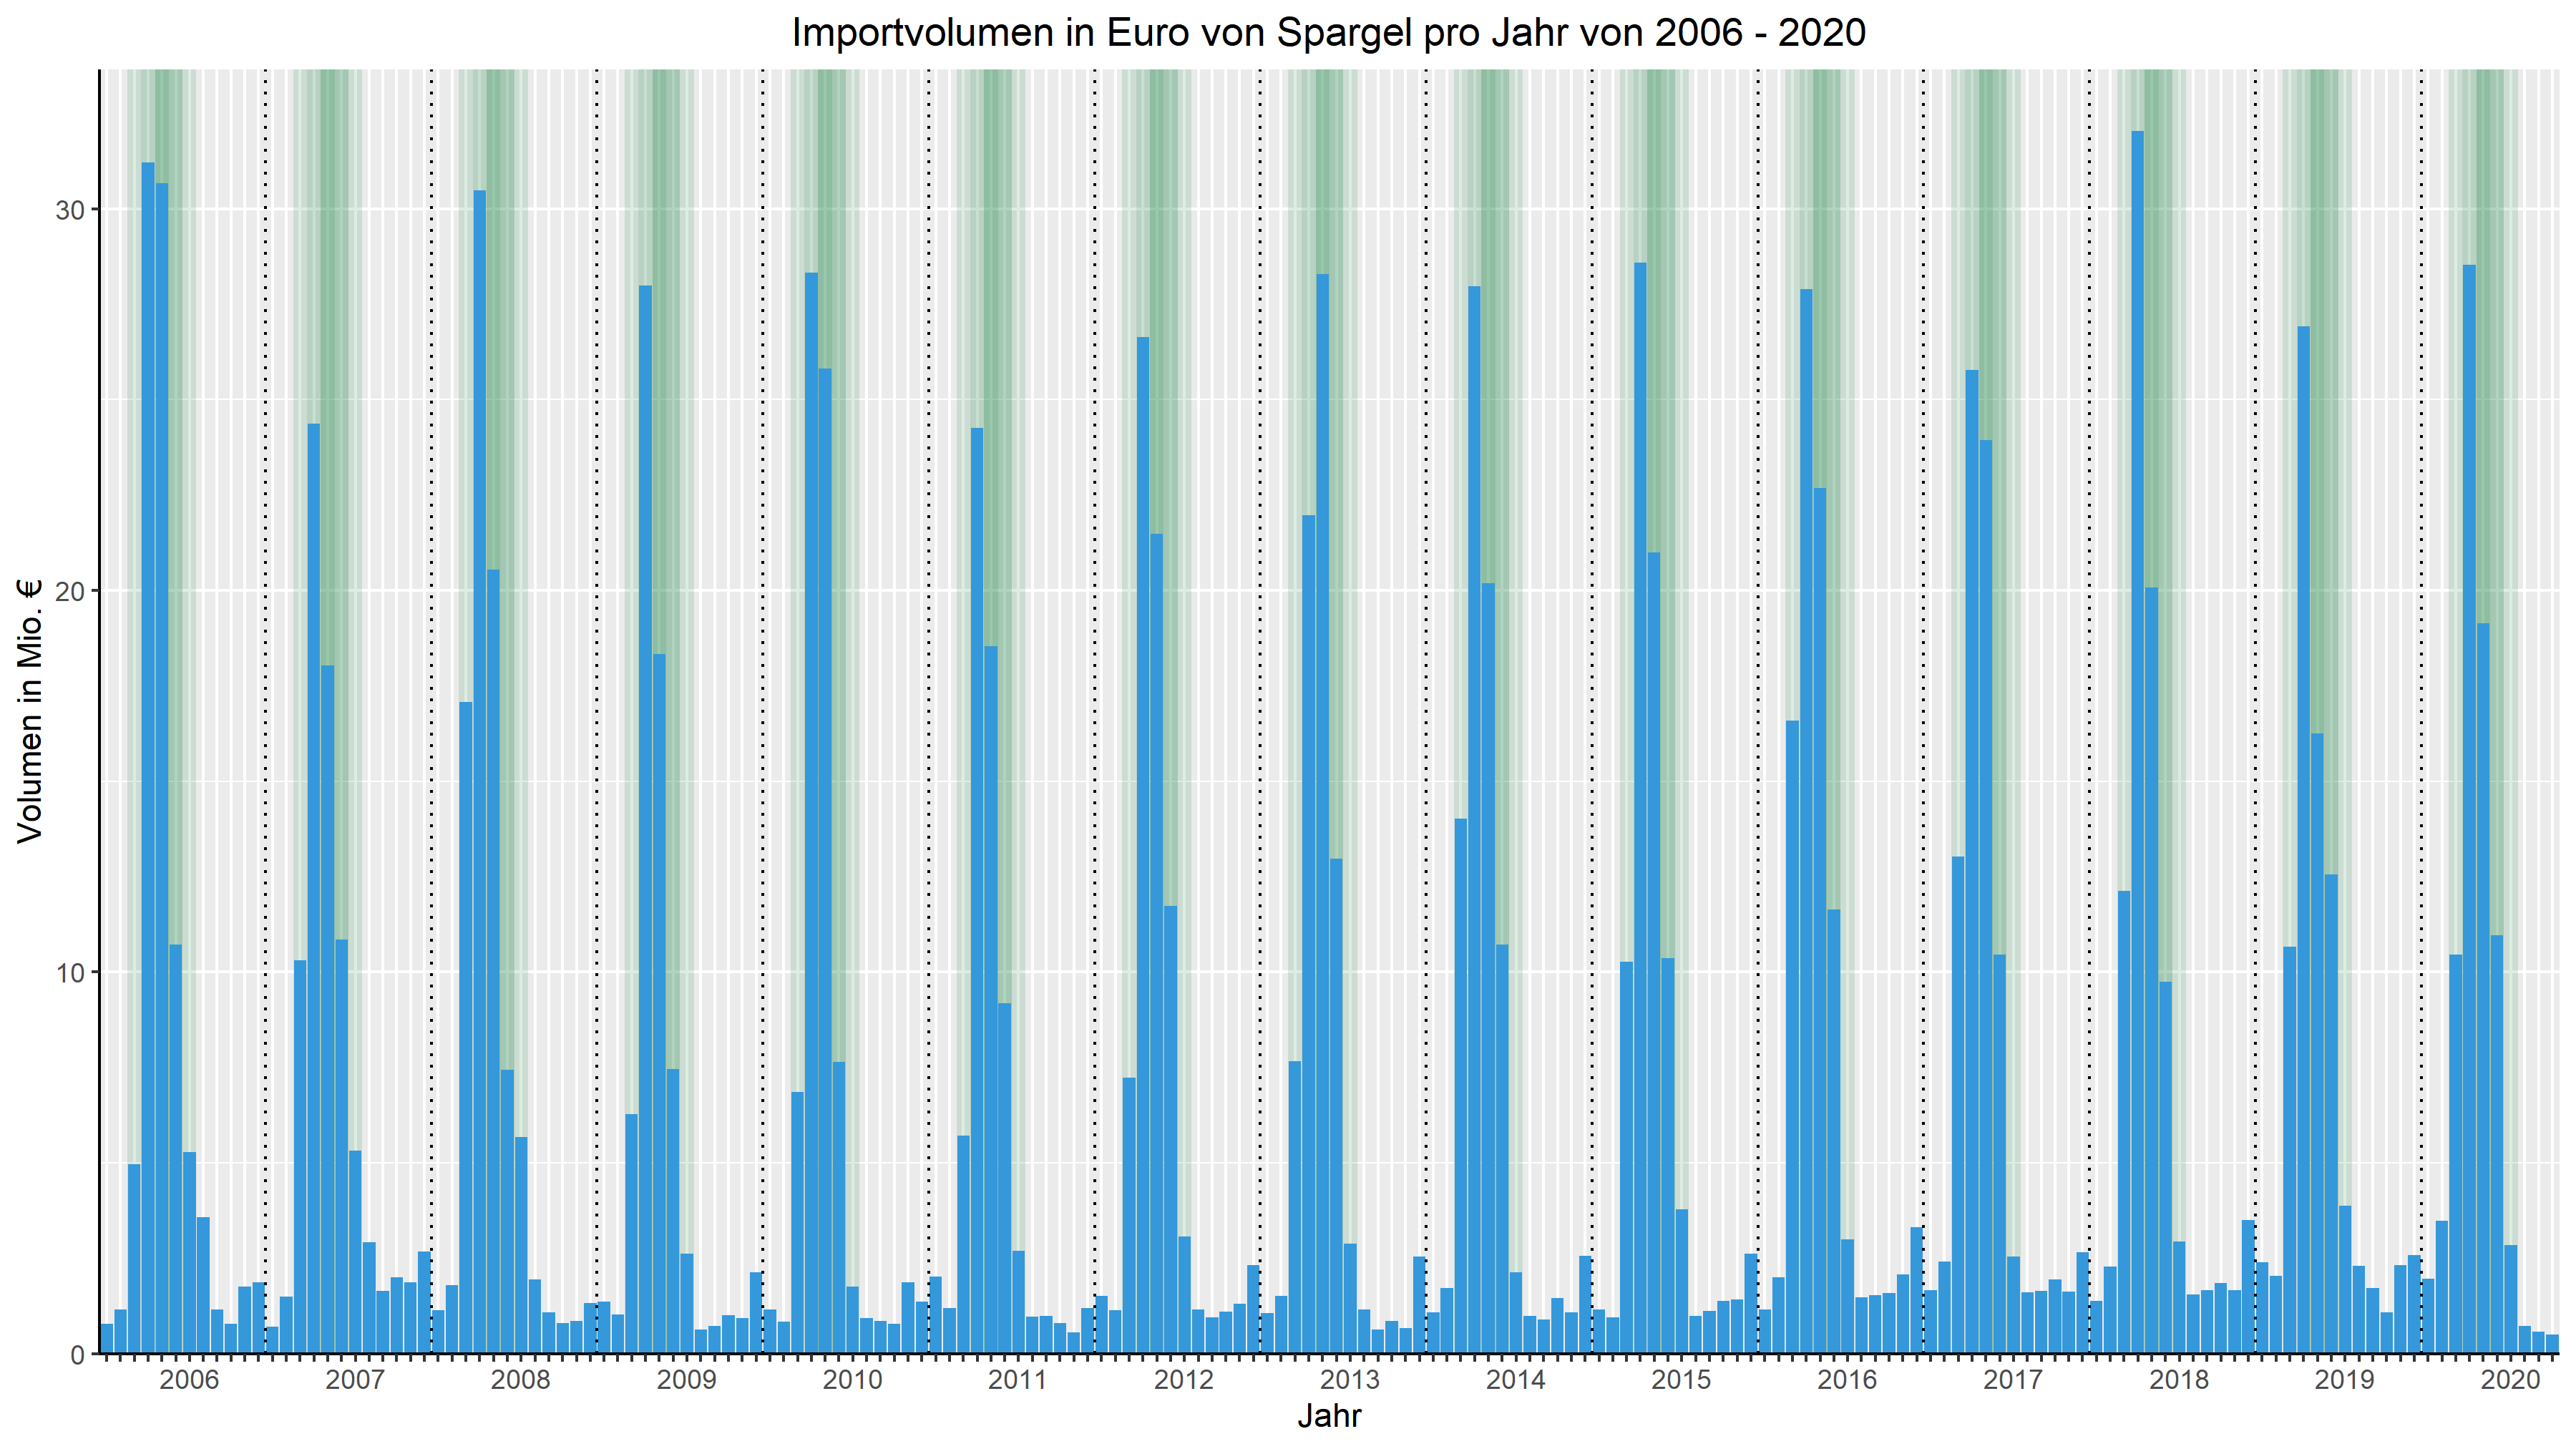
\includegraphics[scale=0.35]{Marco_4_Folie}
	\end{figure}
\end{frame}

\begin{frame}
	\frametitle{Probleme Boxplot}
	\begin{figure}[b]
		\centering
		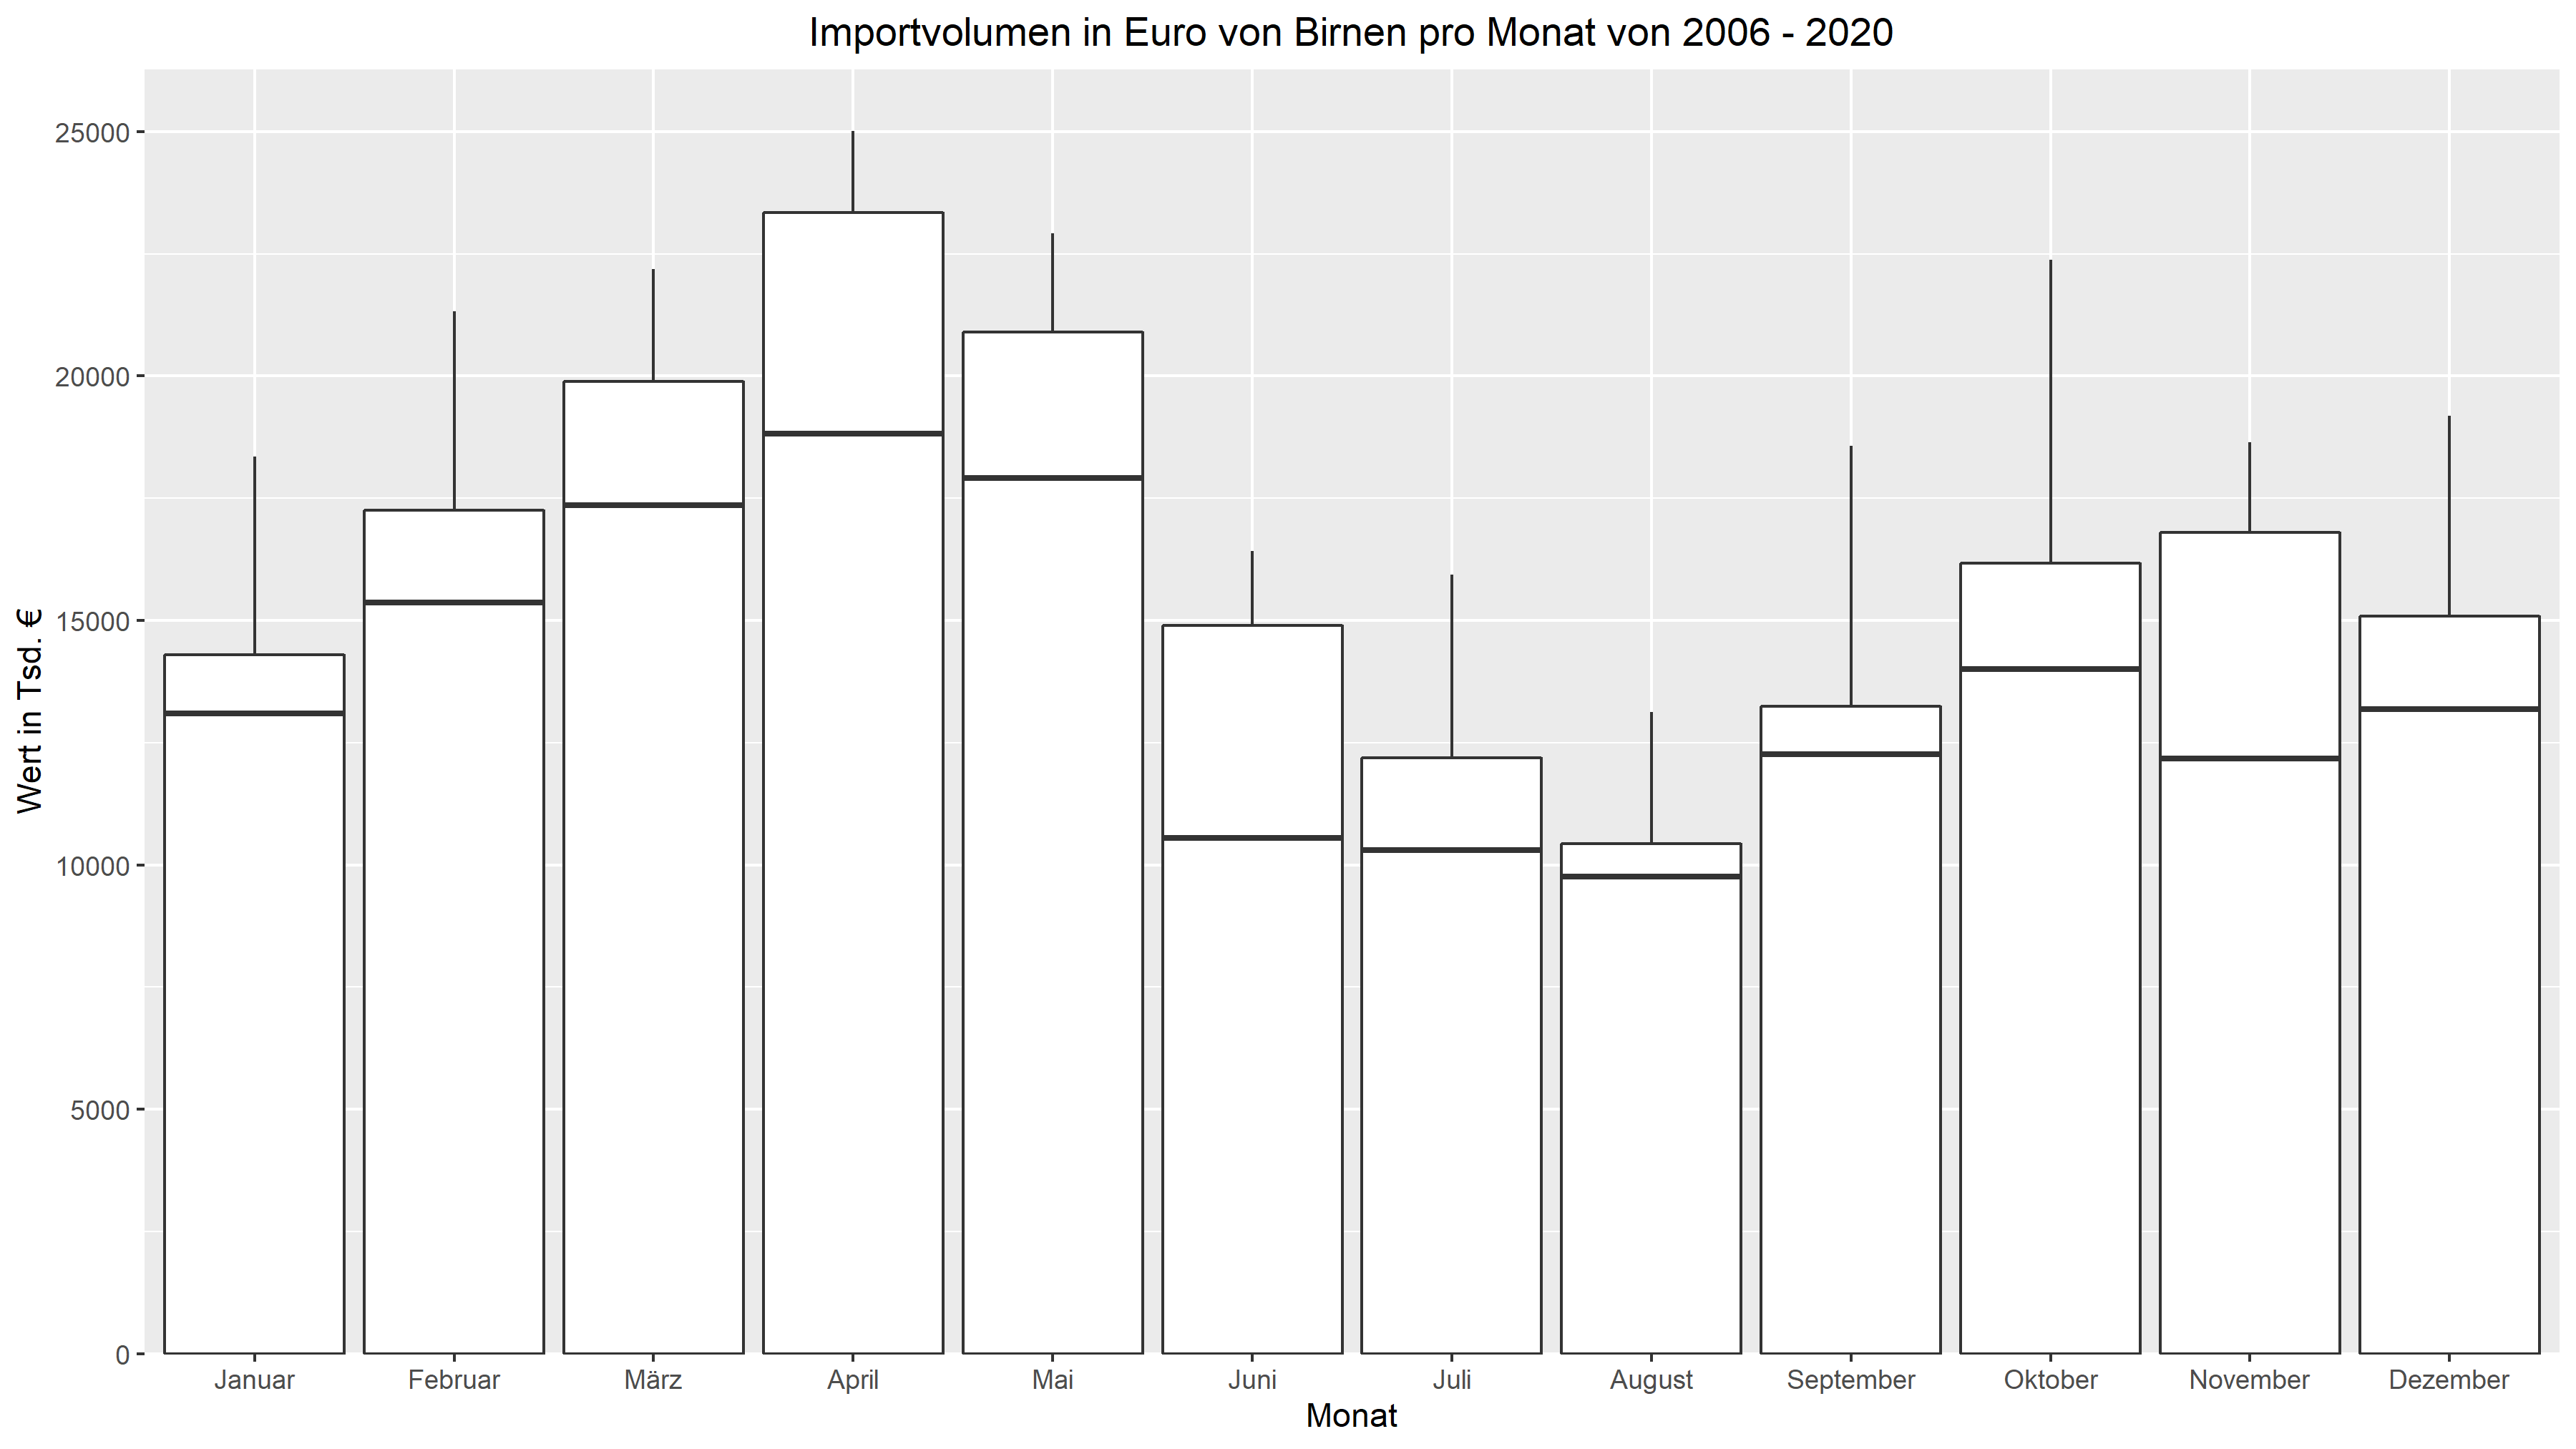
\includegraphics[scale=0.35]{Marco_5_Folie_1}
	\end{figure}
\end{frame}

\begin{frame}
	\frametitle{Probleme Boxplot}
	\begin{figure}[b]
		\centering
		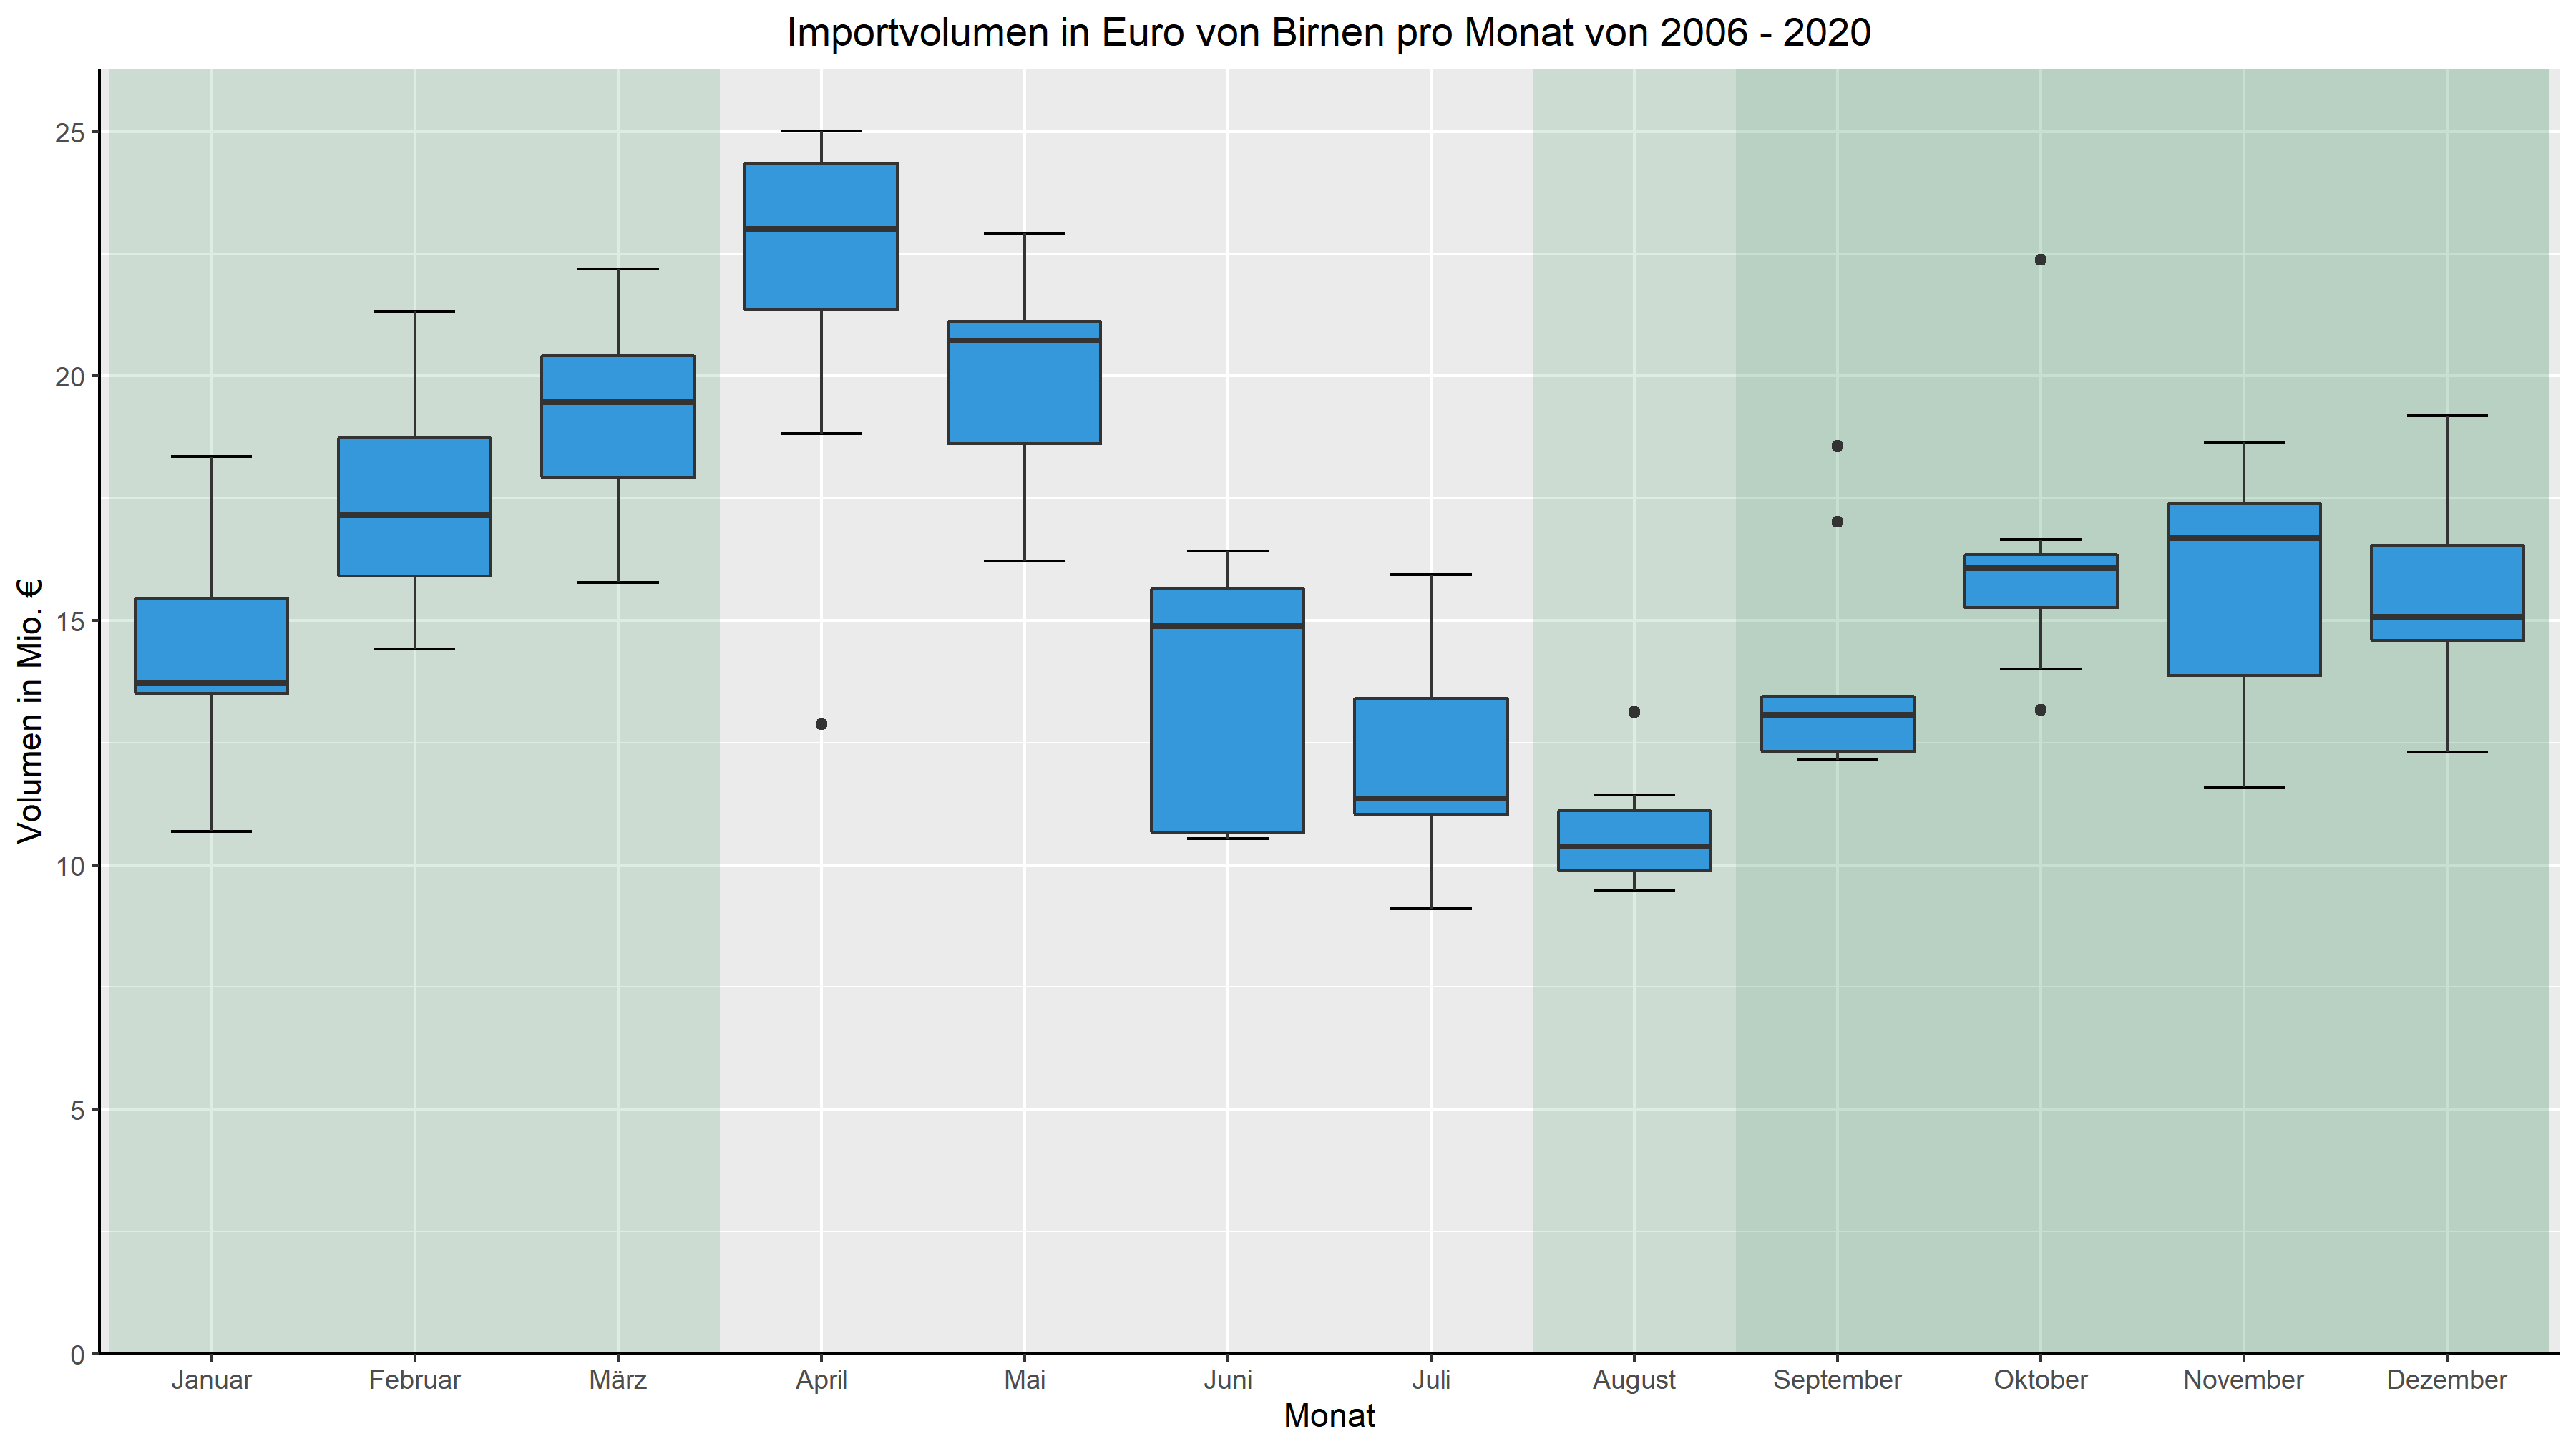
\includegraphics[scale=0.35]{Marco_5_Folie_2}
	\end{figure}
\end{frame}

\begin{frame}
	\frametitle{Boxplot - Ausreißer}
	\begin{figure}[b]
		\centering
		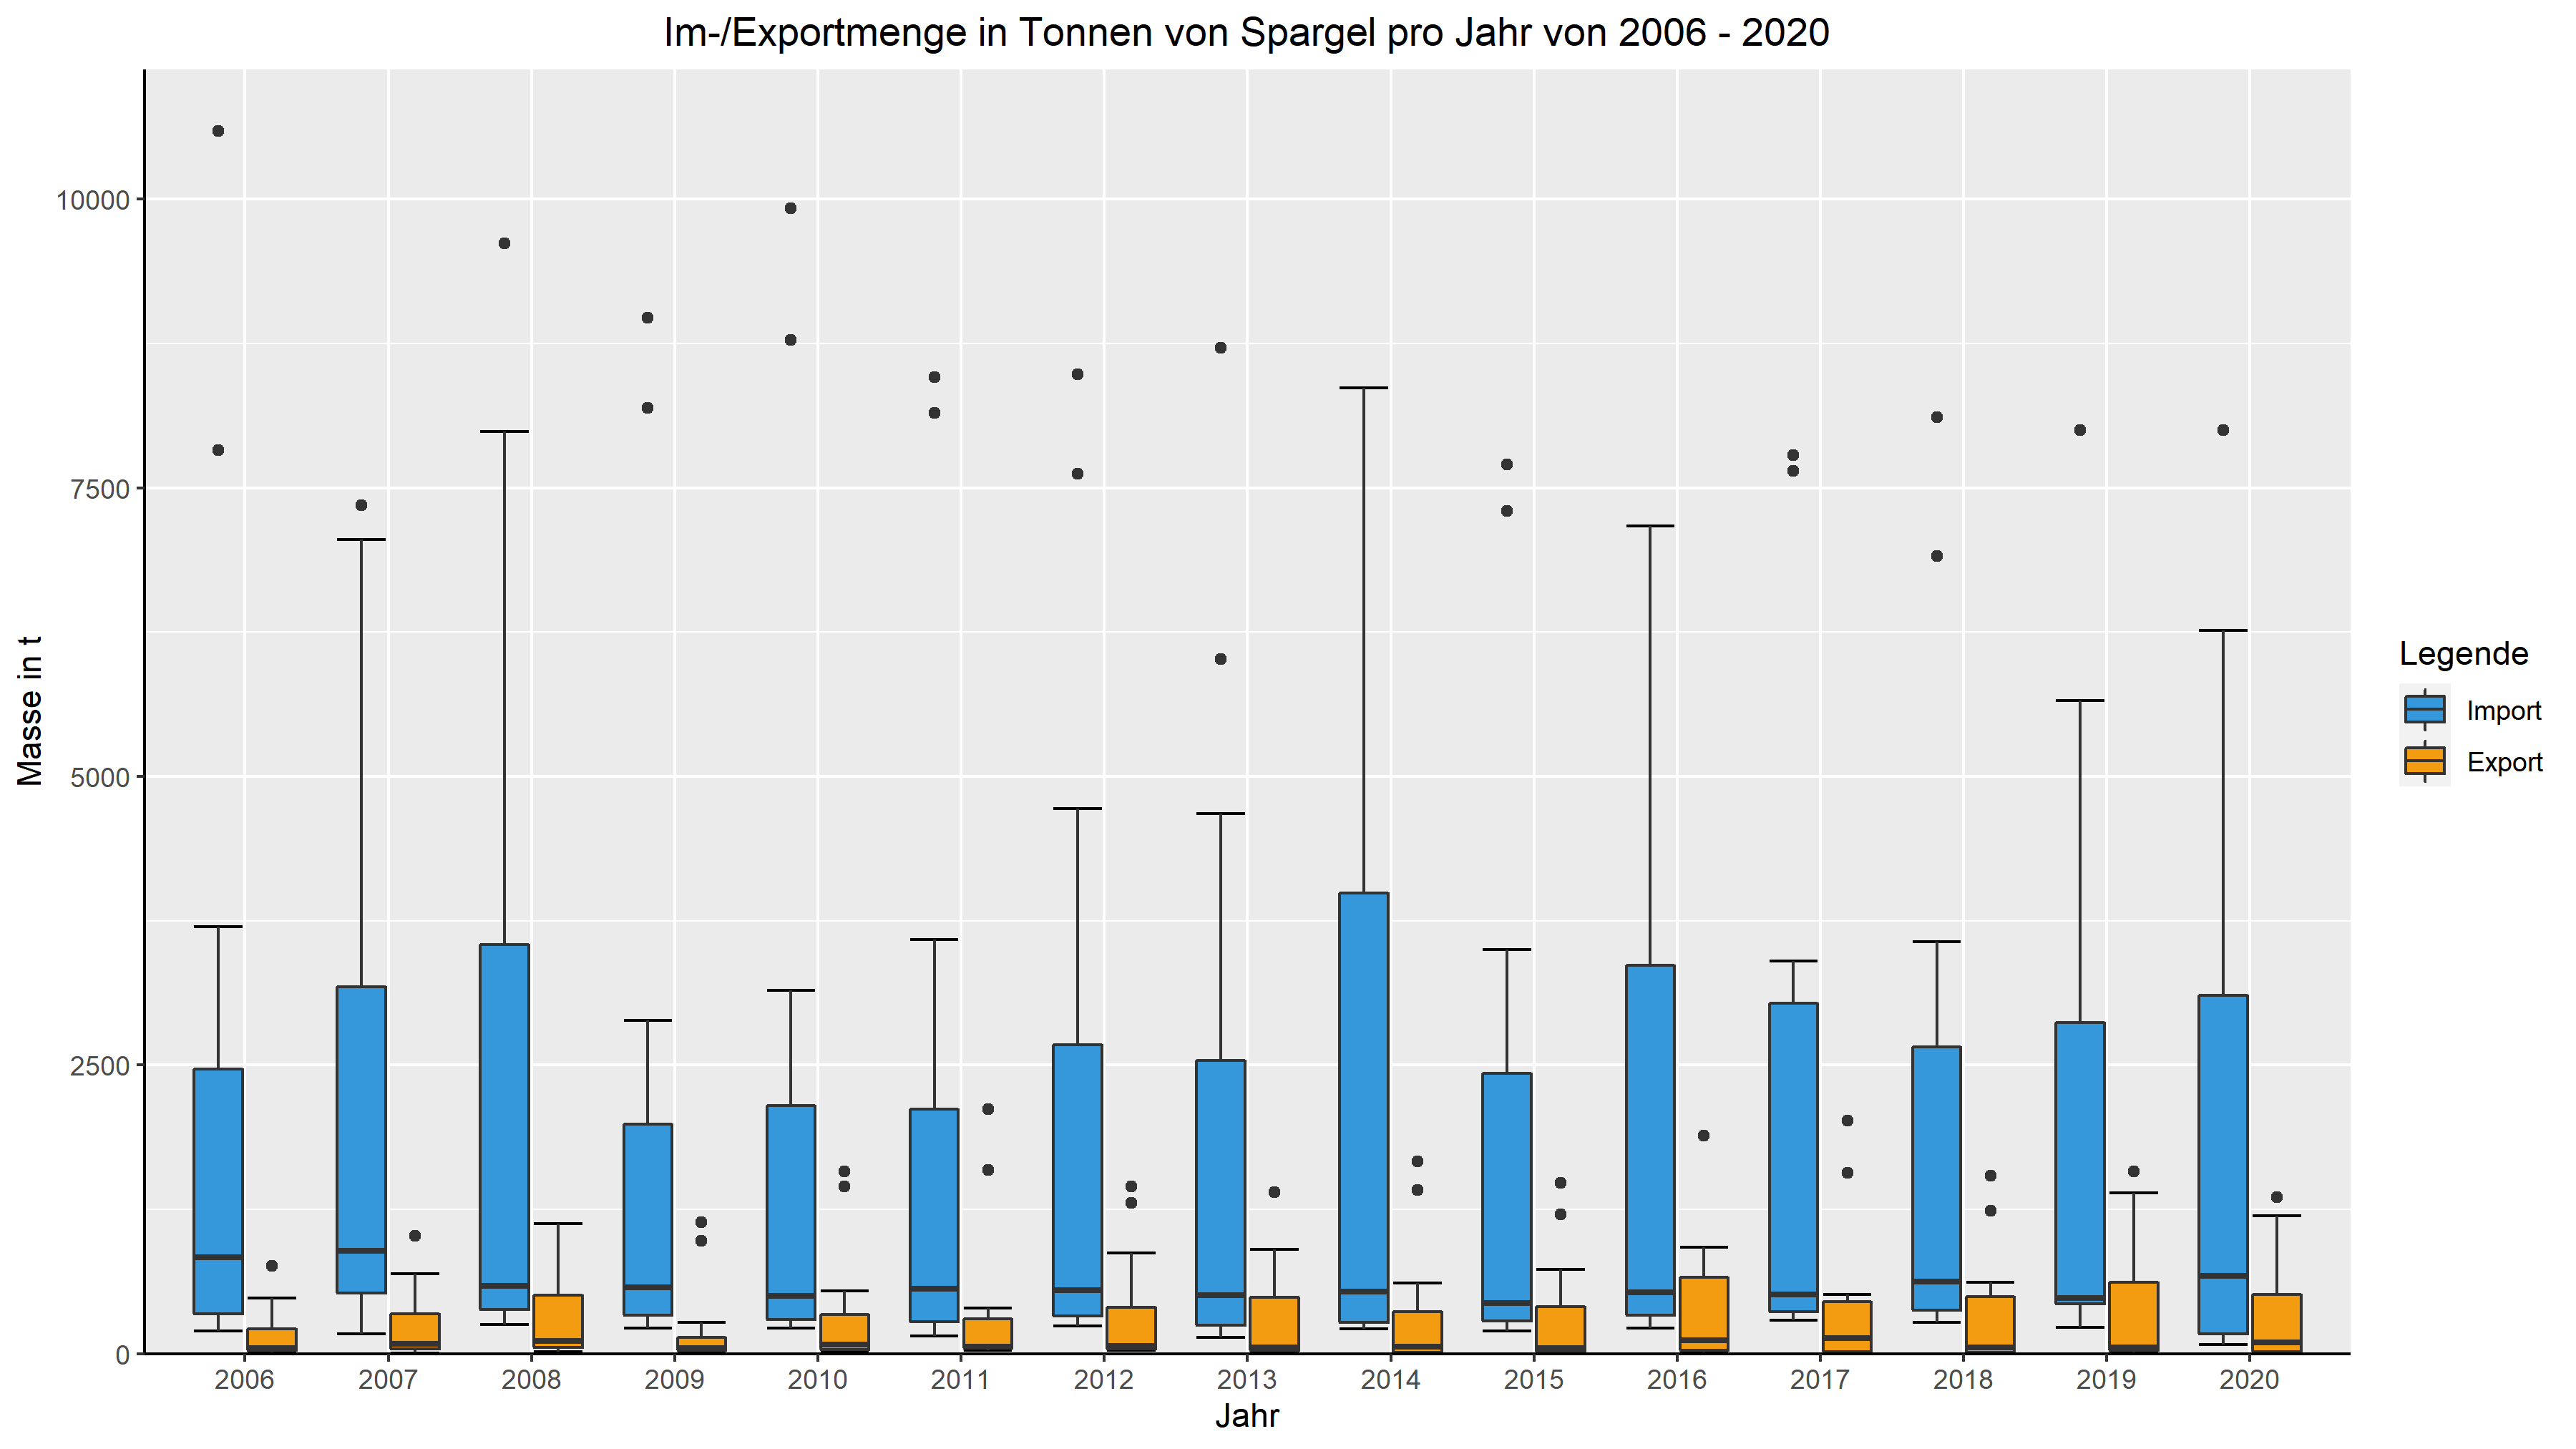
\includegraphics[scale=0.35]{Marco_6_Folie_1}
	\end{figure}
\end{frame}

\begin{frame}
	\frametitle{Boxplot - Ausreißer}
	\begin{figure}[b]
		\centering
		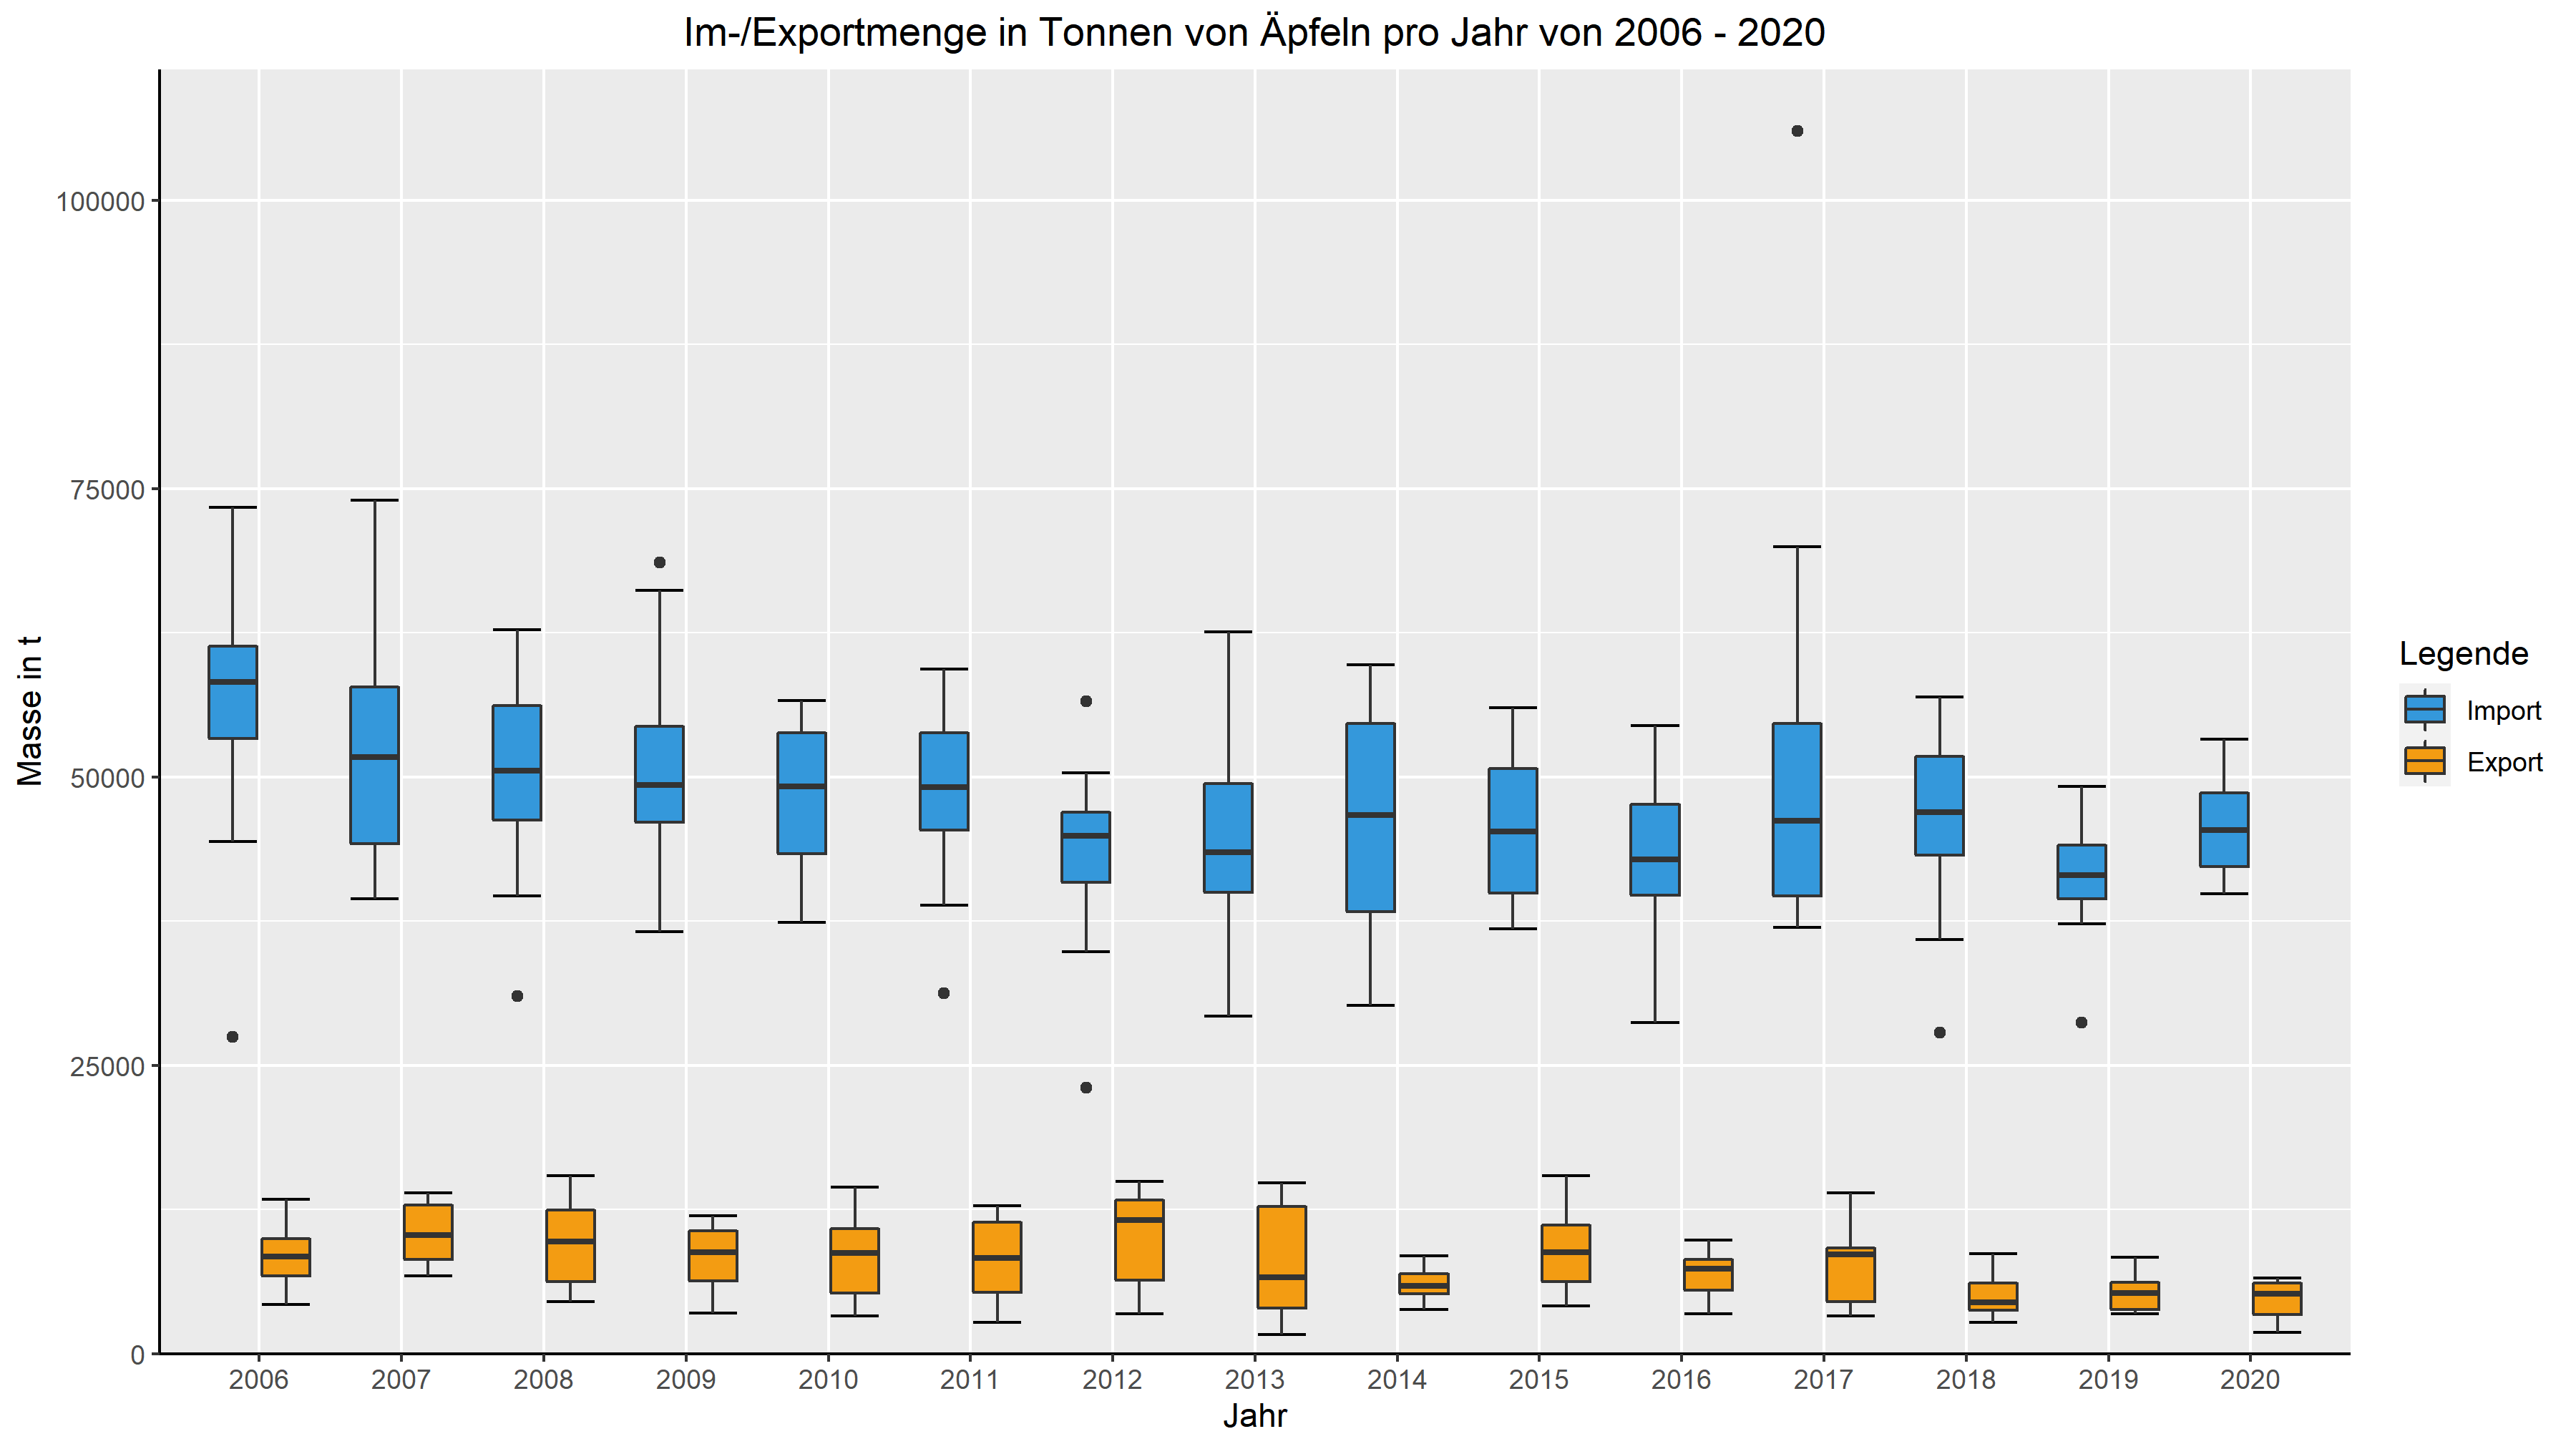
\includegraphics[scale=0.35]{Marco_6_Folie_2}
	\end{figure}
\end{frame}

\section{Sichtung}
\begin{frame}
	\begin{center}
		{\Huge explorative Datensichtung}
	\end{center}
\end{frame}

\begin{frame}
	\frametitle{Kürbisse}
	\begin{figure}[b]
		\centering
		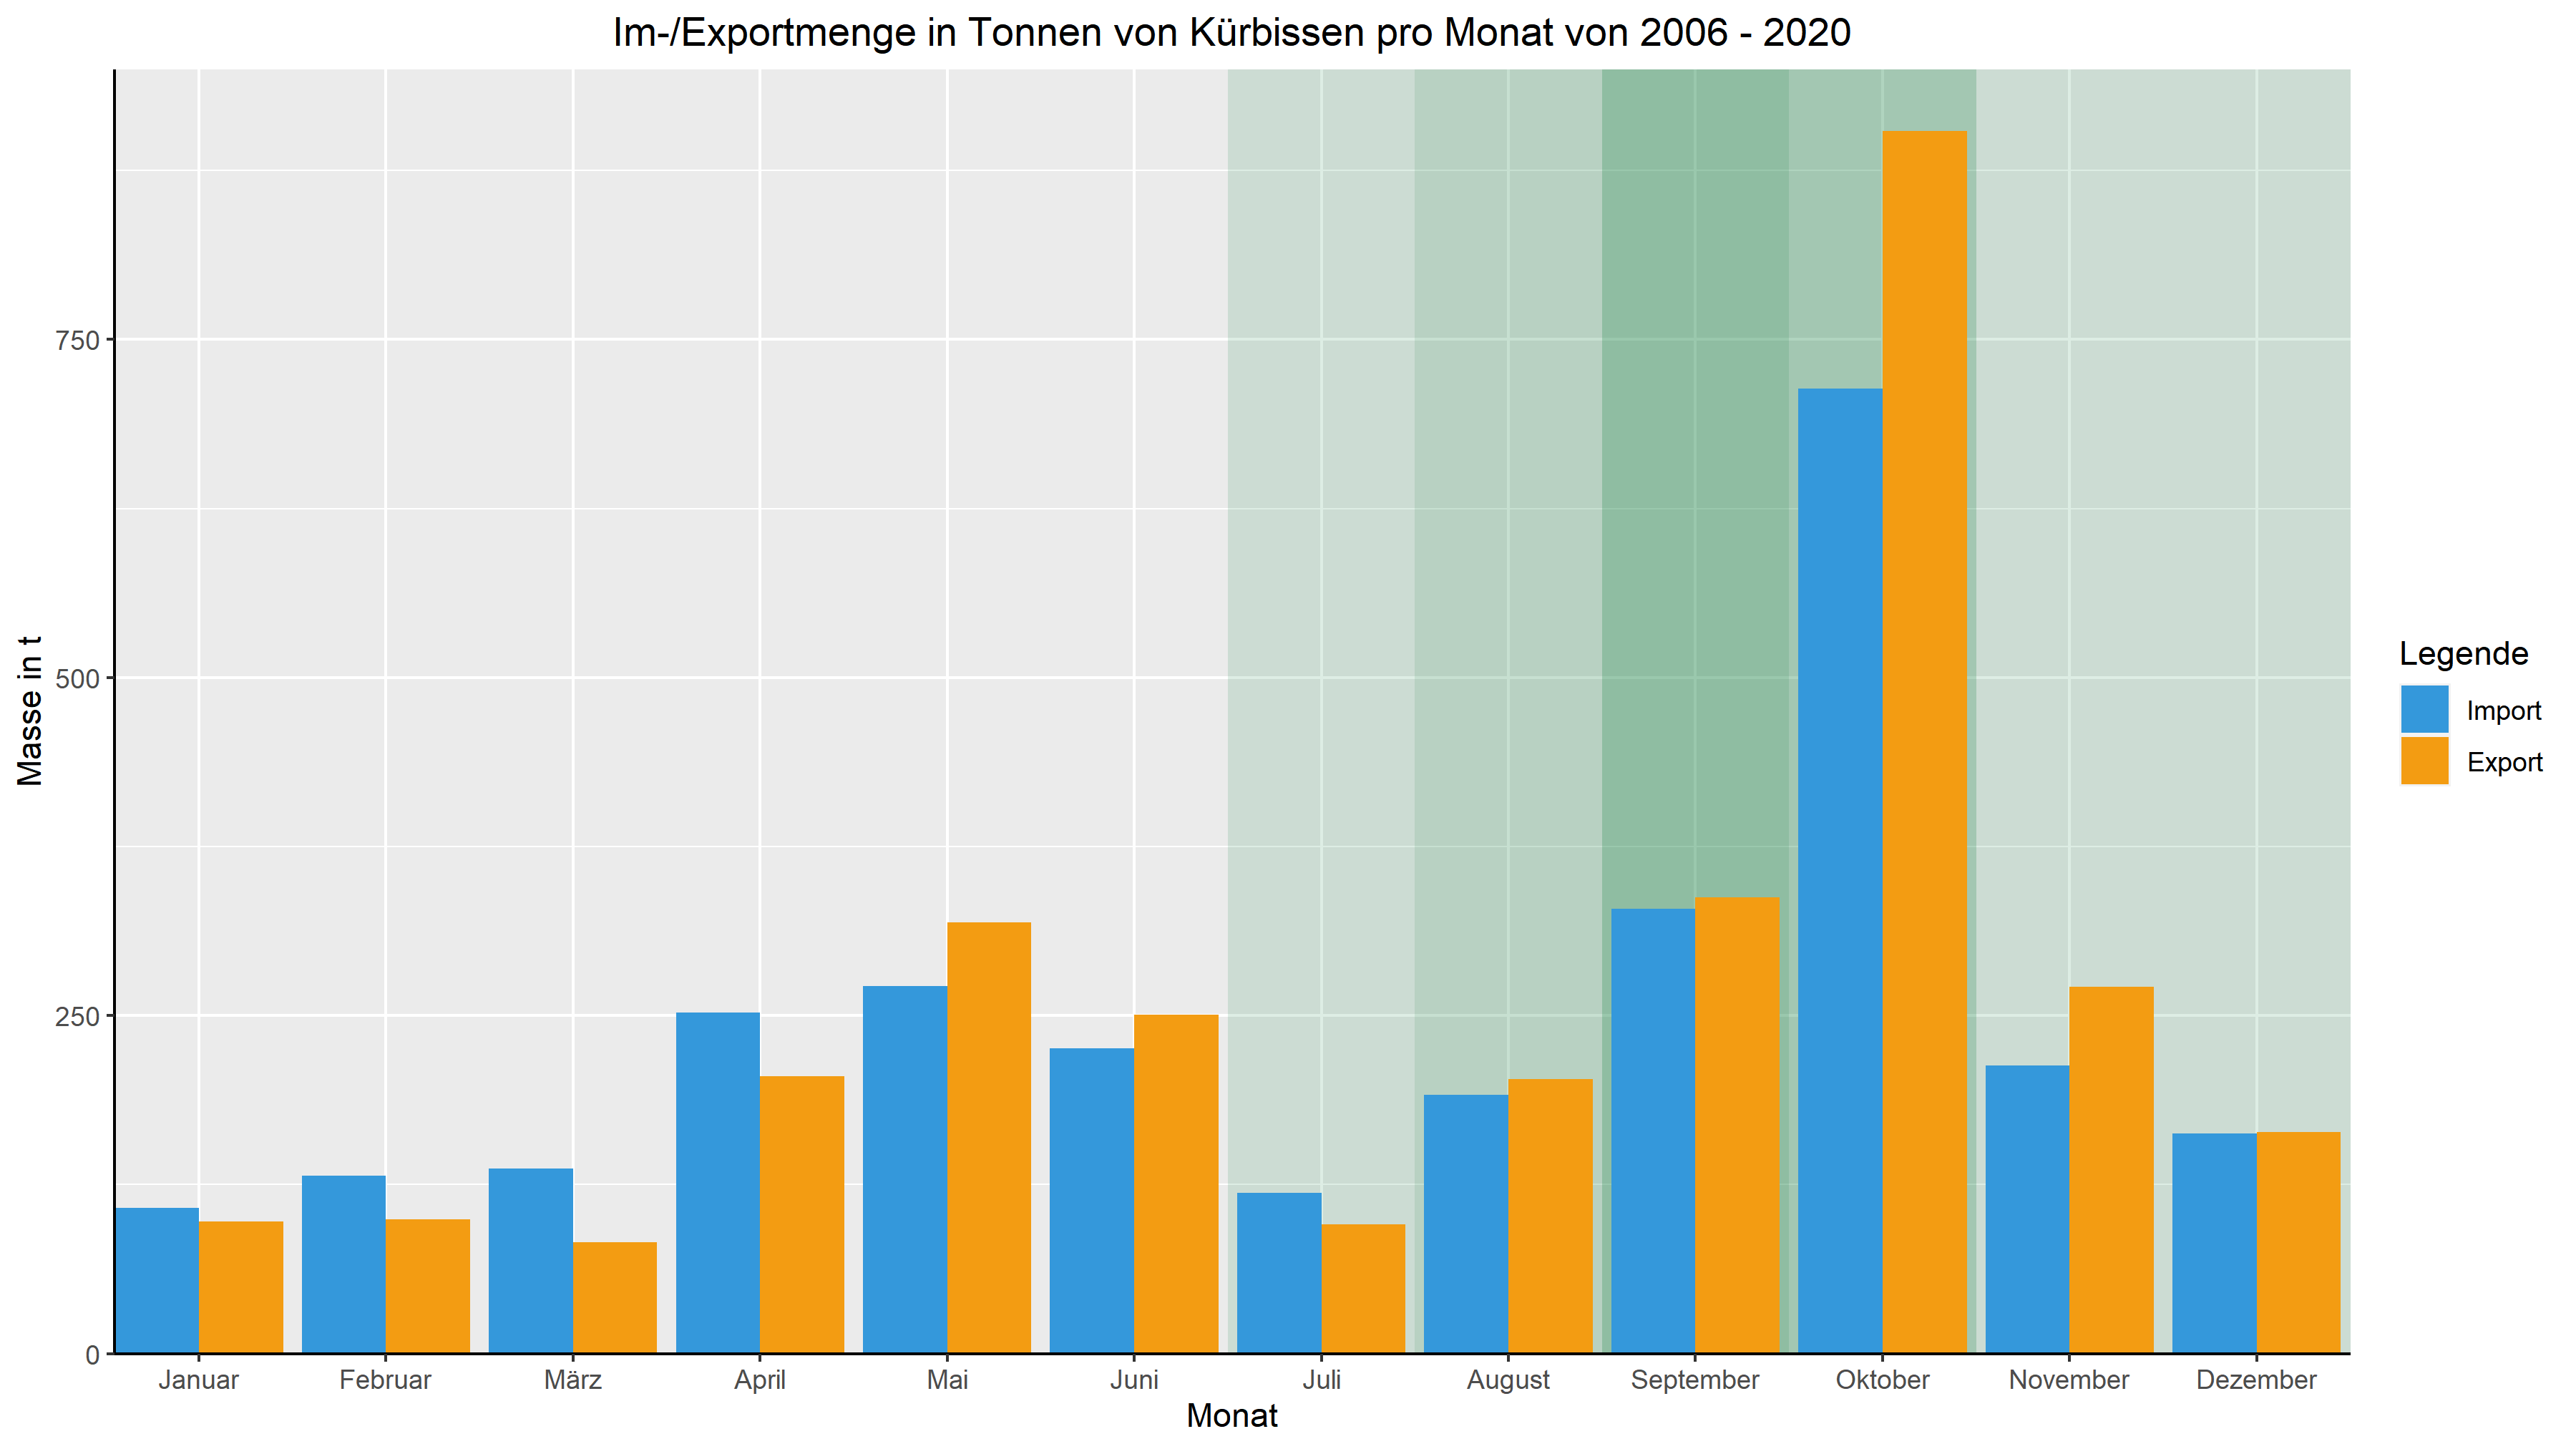
\includegraphics[scale=0.35]{Kuerbissen_monthly_weight_Im-Export}
	\end{figure}
\end{frame}

\begin{frame}
	\frametitle{Kürbisse}
	\begin{figure}[b]
		\centering
		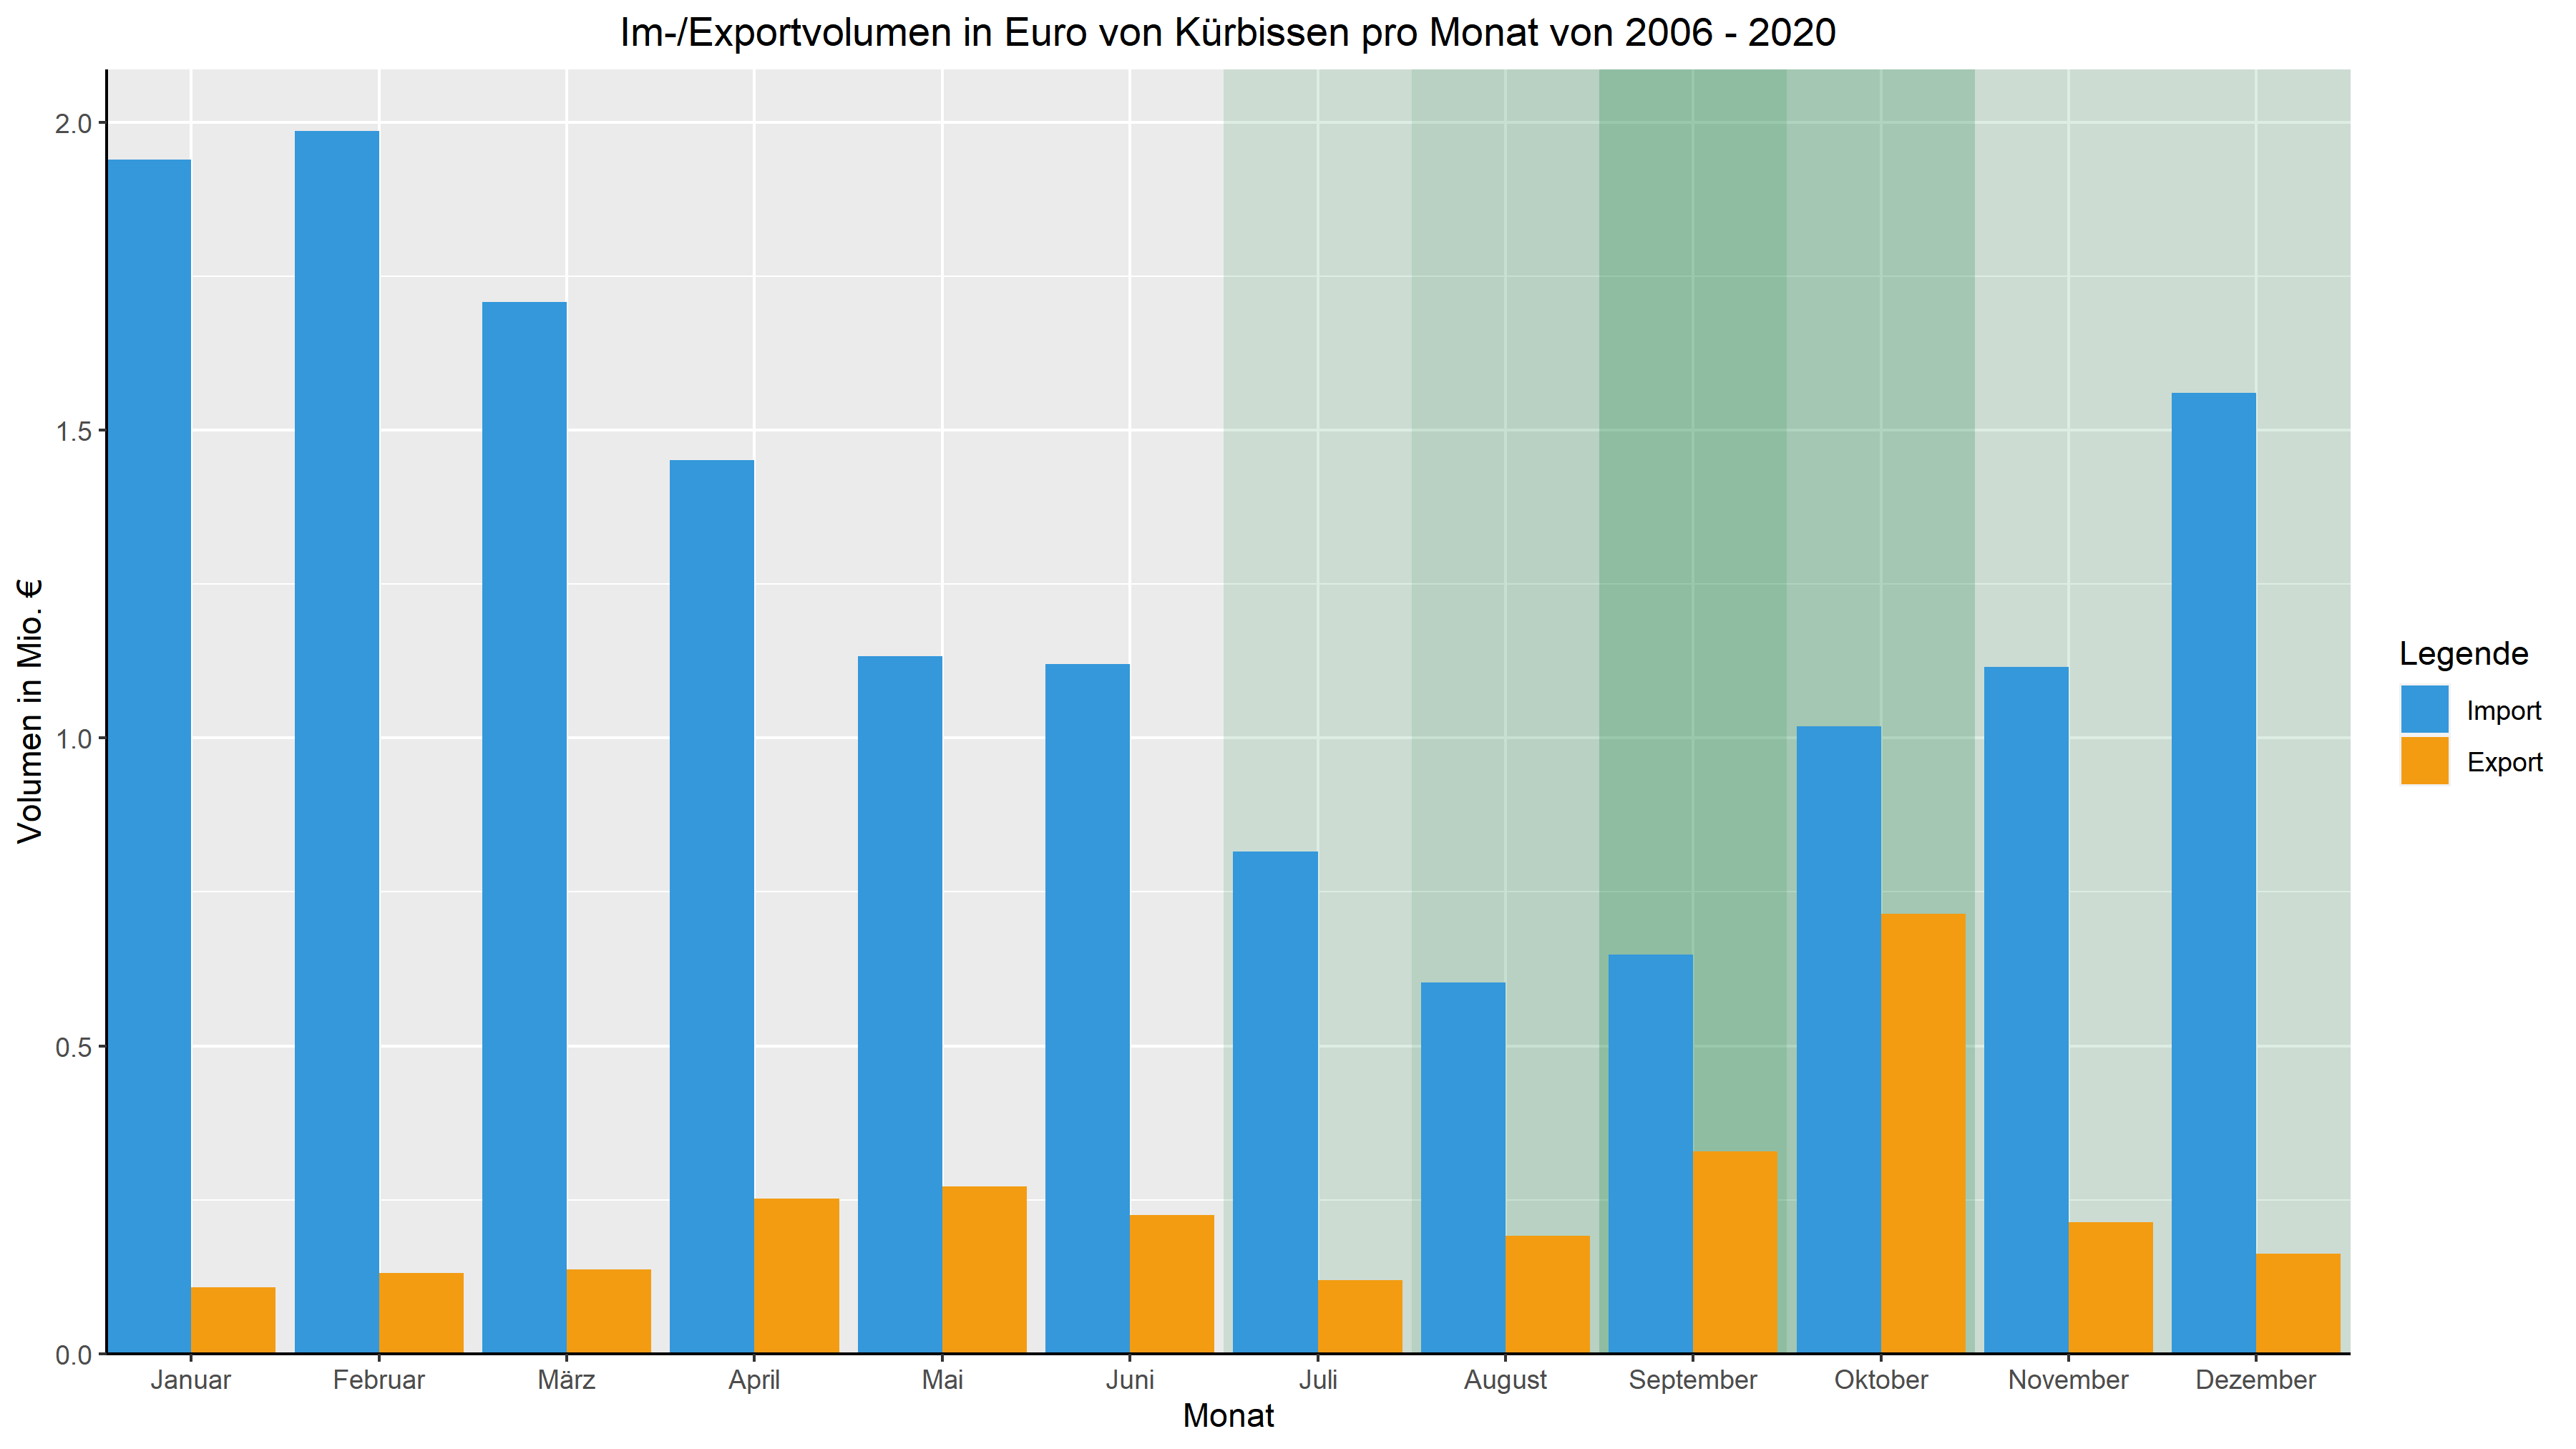
\includegraphics[scale=0.35]{Kuerbissen_monthly_Euro_Im-Export}
	\end{figure}
\end{frame}

\begin{frame}
	\frametitle{Kürbisse}
	\begin{figure}[b]
		\centering
		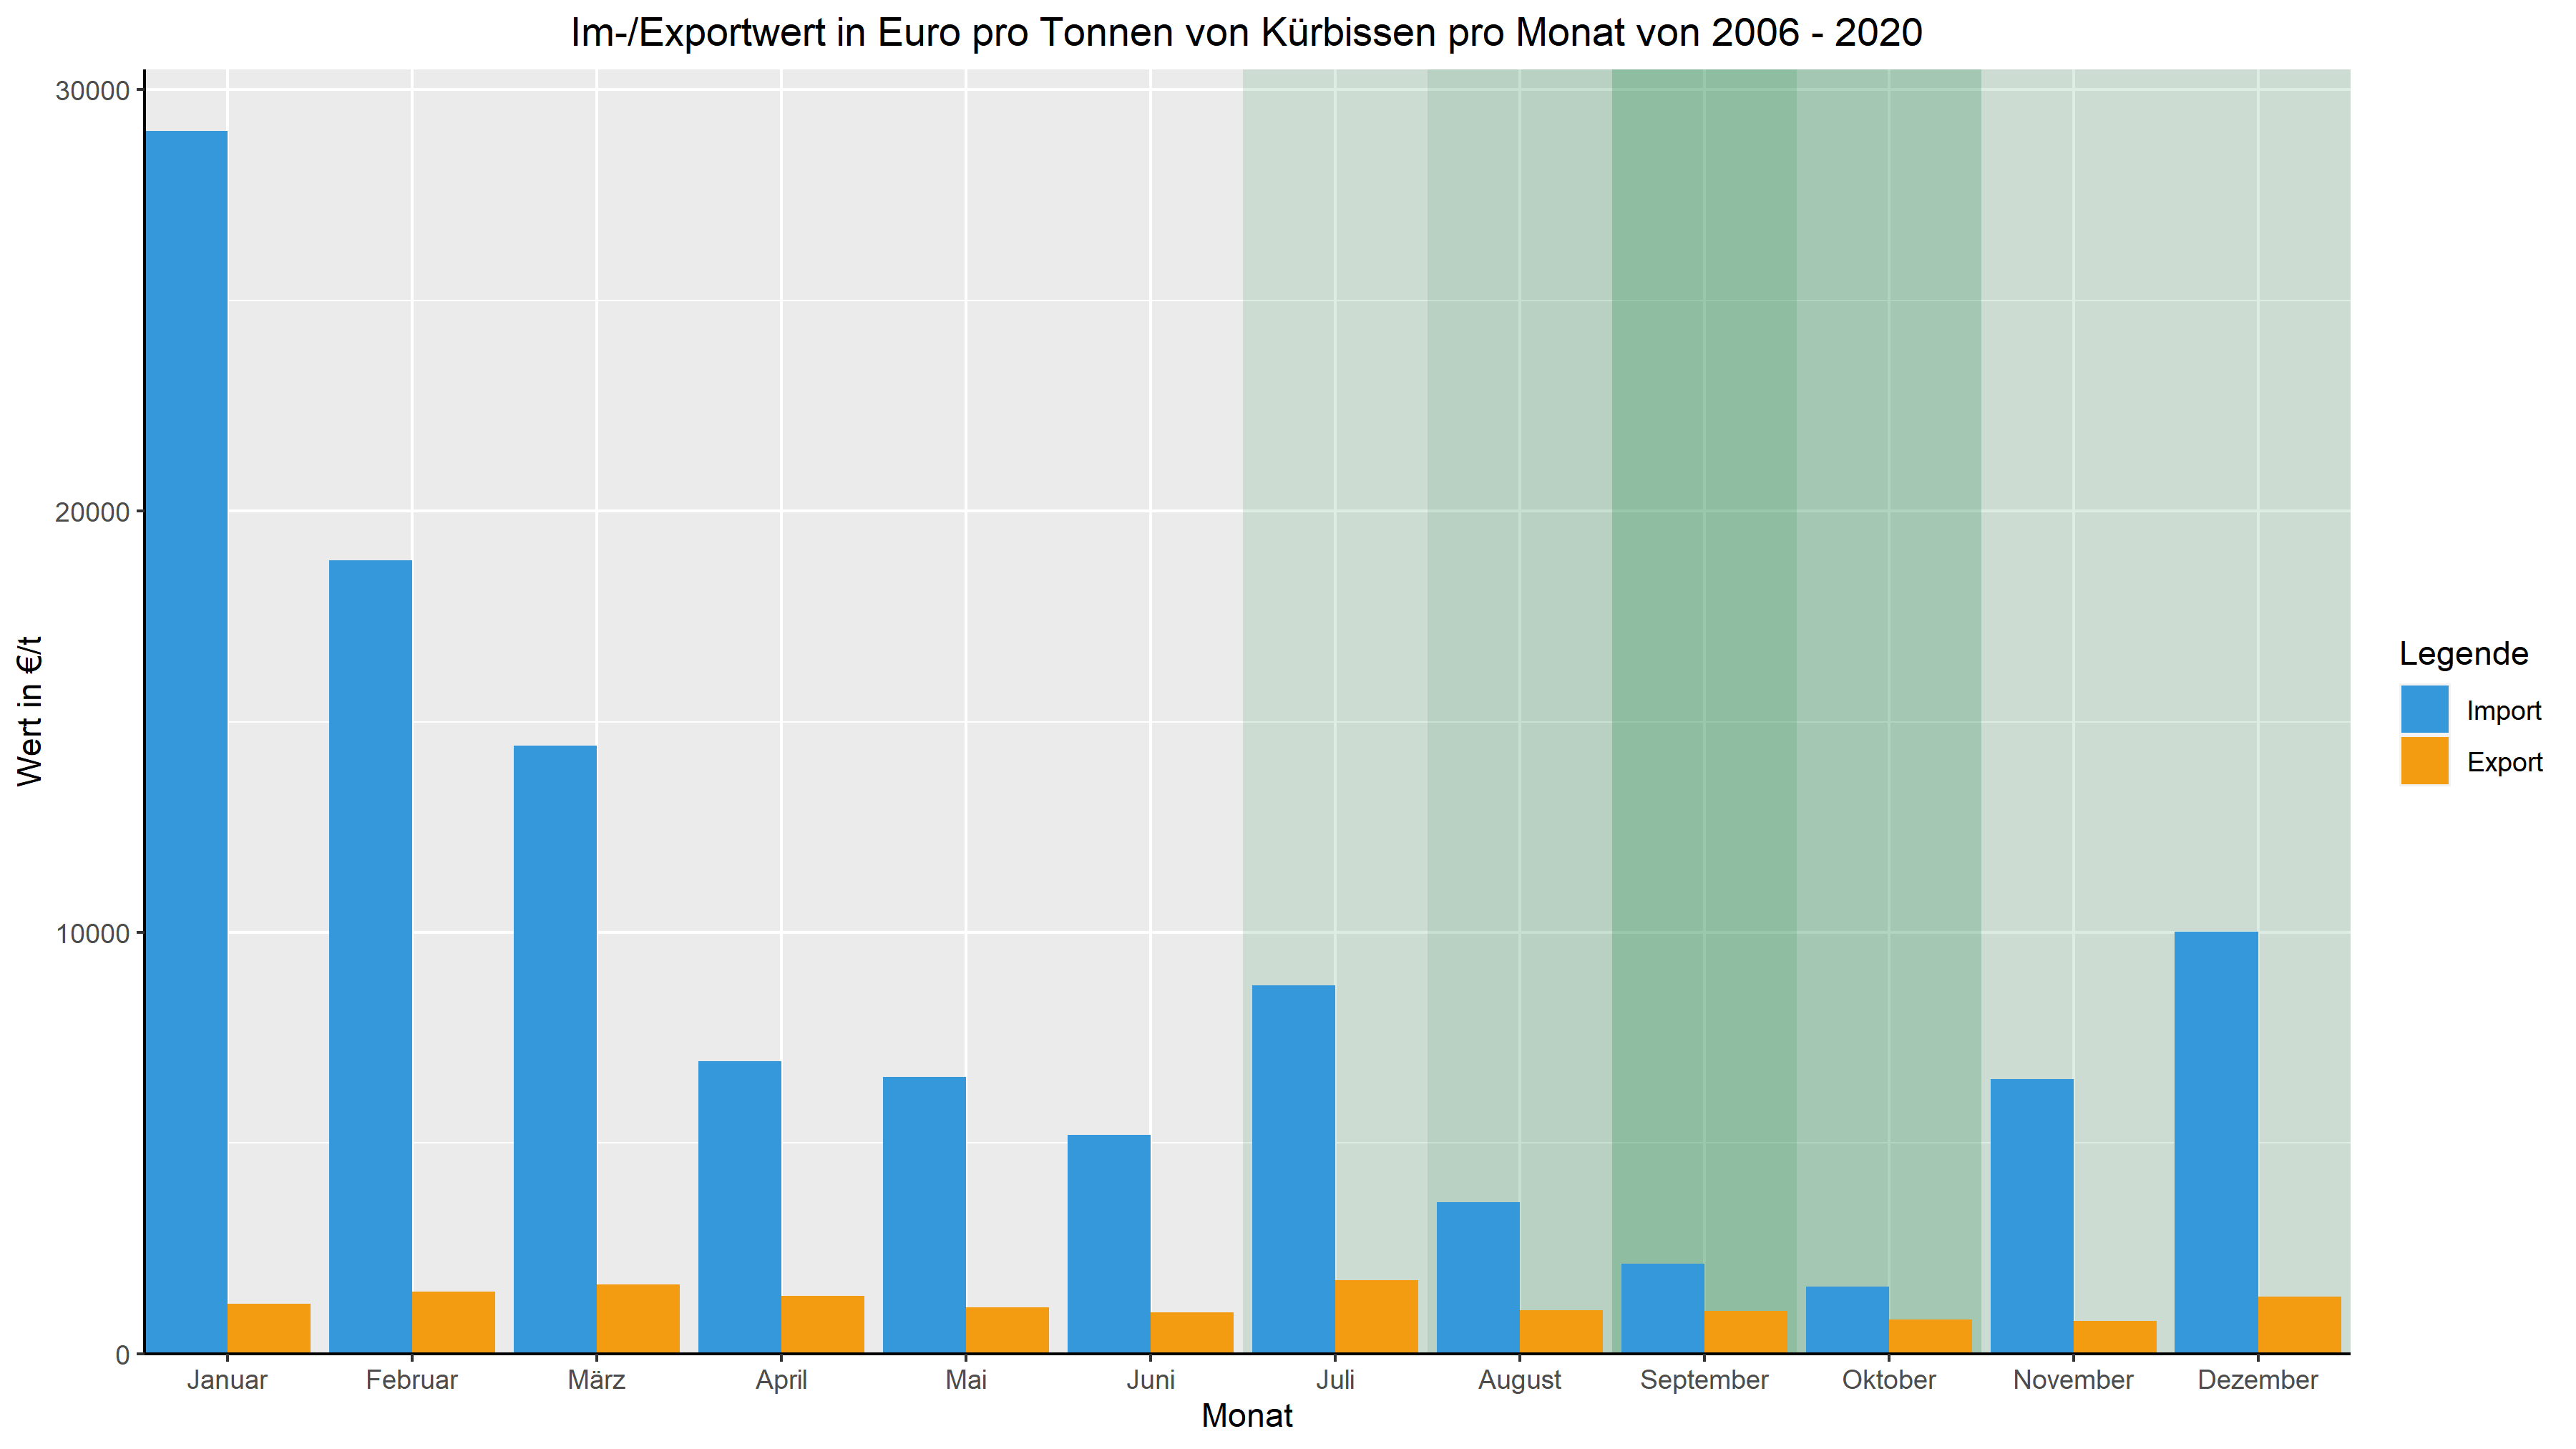
\includegraphics[scale=0.35]{Kuerbissen_monthly_Euro_per_weight_Im-Export}
	\end{figure}
\end{frame}

\section{Fazit}
\begin{frame}
	\frametitle{Fazit}
	\begin{itemize}
		\item Außenhandel beeinflusst durch Saison
		\item bei Produkten mit längerer Saison wenig Beeinflussung
		\item Auswirkungen auf Preis schwanken (noch checken LOL)
	\end{itemize}
\end{frame}

% bibliography
% \break
% \printbibliography

\end{document}
